\subsection{拓扑群中点的邻域}

设 \(\mathfrak{B}\) 为拓扑群 G 中单位元 \(e\) 的邻域滤子，并设 \(a\) 为 G 的任意一点。由于 \(x \to ax\) 与 \(x \to xa\) 都是同胚，因此 \(a\) 的邻域滤子是族 \(a\) . \(\mathfrak{B}\)，即由诸集合 \(a\) . V（其中 V 取遍 \(\mathfrak{B}\)）组成，它同时也是族 \(\mathfrak{B}\) . \(a\)，即由诸集合 V. \(a\) 组成。由此可见，只要知道了群的单位元 \(e\) 的邻域滤子，我们便知道了拓扑群中任意一点的邻域滤子。

如果我们说 \(xy\) 与 \(x^{-1}\) 在 \(x = y = e\) 处连续，就得到（第一章 § 2 第 1 目）：

\((\mathbf{GV}_{\mathbf{I}})\). 对任意 \(\mathbf{U} \in \mathfrak{B}\)，存在 \(\mathbf{V} \in \mathfrak{B}\) 使 \(\mathbf{V} \cdot \mathbf{V} \subset \mathbf{U}\)。

\((\mathbf{GV}_{\mathbf{II}})\). 对任意 \(\mathbf{U}\in \mathfrak{B},\) 有 \(\mathbf{U}^{-1}\in \mathfrak{B}\)

任何滤子 \(\mathfrak{B}\)，只要它在 \(G\) 上并且满足 \((\mathrm{GV}_{\mathbb{I}})\) 与 \((\mathrm{GV}_{\mathbb{II}})\)，便也满足 \((\mathrm{GV}_{\alpha})\)：对任意 \(U \in \mathfrak{B}\)，存在 \(V \in \mathfrak{B}\) 使 \(V \cdot V^{-1} \subset U\)。因为由 \((\mathrm{GV}_{\mathbb{I}})\)，存在 \(W \in \mathfrak{B}\) 使 \(W \cdot W \subset U\)；又由 \((\mathrm{GV}_{\mathbb{II}})\)，存在 \(V \in \mathfrak{B}\) 使 \(V \subset W \cap W^{-1}\)；于是 \(V^{-1} \subset W\)，从而 \(V \cdot V^{-1} \subset W \cdot W \subset U\)。

反之，设 \(\mathfrak{B}\) 为 \(\mathbf{G}\) 上满足 \((\mathrm{GV}_{\alpha})\) 的一个滤子，则首先可知 \(e\) 属于每个集合 \(\mathbf{U} \in \mathfrak{B}\)；因为若 \(\mathbf{V} \in \mathfrak{B}\) 使 \(\mathbf{V} \cdot \mathbf{V}^{-1} \subset \mathbf{U}\)，则由于 V 非空，我们有 \(x.x^{-1}=e\in U\)，它对每个 \(x\in V\) 成立。于是条件 \((\mathrm{GV}_{\alpha})\) 蕴含 \(V^{-1}\subset V.V^{-1}\subset U\)，因而 \(U^{-1}\in\mathfrak{B}\)（只要 \(U\in\mathfrak{B}\)）。最后，若 \(V\in\mathfrak{B}\) 使 \(V.V^{-1}\subset U\)，且 \(W\in\mathfrak{B}\) 使 \(W\subset V\cap V^{-1}\)，则 \(W.W\subset U\)。由此可见，\((\mathrm{GV}_{\alpha})\) 等价于 \((\mathrm{GV}_{I})\) 与 \((\mathrm{GV}_{II})\) 的合取。

最后，由于 \(x \rightarrow axa^{-1}\) 是使 e 固定不动的同胚，B 具有下列性质：

\((\mathrm{GV}_{\mathrm{III}})\). 对所有 \(a \in \mathbf{G}\) 与所有 \(\mathbf{V} \in \mathfrak{B}\)，有 \(a. \mathbf{V}.a^{-1} \in \mathfrak{B}\)。

滤子 \(\mathfrak{B}\) 的这三个性质是特征性质：

命题 1 设 G 是一个群，B 是 G 上满足公理 \((\mathrm{GV}_{\mathrm{I}})\)、\((\mathrm{GV}_{\mathrm{II}})\) 与 \((\mathrm{GV}_{\mathrm{III}})\) 的一个滤子。则在 G 上存在唯一的与 G 的群结构相容的拓扑，使 B 是单位元 e 的邻域滤子。对这个拓扑，任一点 \(a \in G\) 的邻域滤子与两个滤子 a.B 和 B.a 中的每一个都相同。

如果存在具有所需性质的拓扑，那么由上文所述，\(a\) 的邻域滤子与两个滤子 \(a\) . \(\mathfrak{B}\) 和 \(\mathfrak{B}.a\) 中的每一个都重合；因此，如果这样的拓扑存在，它便是唯一的。只要证明 1) 诸滤子 \(a\) . \(\mathfrak{B}\) 是 \(\mathbf{G}\) 上某个拓扑的邻域滤子，以及 2) 这个拓扑与 \(\mathbf{G}\) 的群结构相容，存在性便得证。

\begin{enumerate}
\def\labelenumi{\arabic{enumi})}
\item
  滤子 \(a. \mathfrak{B}\) 满足公理 \((\mathrm{V}_{\mathrm{III}})\)（见第一章 § 1 第 2 目），这由 \((\mathrm{GV}_{\mathrm{I}})\) 与 \((\mathrm{GV}_{\mathrm{II}})\) 推出，我们前面已经看到；因此，要证明 \(a. \mathfrak{B}\) 是 \(a\) 在 \(G\) 上一个拓扑中的邻域滤子，只需验证公理 \((\mathrm{V}_{\mathrm{IV}})\)。设 \(V\) 是 \(\mathfrak{B}\) 中任一集合，\(W\) 是 \(\mathfrak{B}\) 中使 \(W.W \subset V\) 的一个集合；则对任意 \(x \in a.W\)，有 \(x.W \subset a.W.W \subset a.V\)，于是 \(a.V\) 属于滤子 \(x. \mathfrak{B}\)；因而 \((\mathrm{V}_{\mathrm{IV}})\) 得到满足。
\item
  我们现在证明由邻域滤子 \(a\) . \(\mathfrak{B}\) 所定义的拓扑满足 (GT')。设 \(a, b\) 是 G 的任意两点；若令 \(x = au\)、\(y = bv\)，则我们要证明：\(xy^{-1}\) 可以随意地接近 \(ab^{-1}\)，只要 \(u\) 与 \(v\) 充分接近 \(e\)。现在 \((ab^{-1})^{-1}(xy^{-1}) = buv^{-1}b^{-1}\)；设 U 是 \(e\) 的任一邻域，则我们将有 \(buv^{-1}b^{-1} \in U\)，只要 \(uv^{-1} \in b^{-1}Ub = V\)，并且 \(V \in \mathfrak{B}\)（由 \((\mathrm{GV}_{\mathrm{III}})\)）。但由 \((\mathrm{GV}_{\mathrm{I}})\) 与 \((\mathrm{GV}_{\mathrm{II}})\)，存在 \(W \in \mathfrak{B}\) 使 \(W.W^{-1} \subset V\)；因此只需取 \(u \in W\) 与 \(v \in W\)，便有 \(xy^{-1} \in (ab^{-1})U\)。证毕。
\end{enumerate}

在 G 上定义一个与群结构相容的拓扑，一个常用方法是给出一个满足公理 \((\mathrm{GV}_{\mathrm{I}})\)、\((\mathrm{GV}_{\mathrm{II}})\) 与 \((\mathrm{GV}_{\mathrm{III}})\) 的滤子。对于滤子基 B，相应的条件如下：

\((\mathbf{GV}_{\mathbf{I}}^{\prime})\). 对任意 \(\mathbf{U}\in \mathfrak{B}\)，存在 \(\mathbf{V}\in \mathfrak{B}\) 使 \(\mathbf{V}.\mathbf{V}\subset \mathbf{U}\)。\((\mathrm{GV}_{\mathrm{II}}^{\prime})\). 对任意 \(\mathbf{U} \in \mathfrak{B}\)，存在 \(\mathbf{V} \in \mathfrak{B}\) 使 \(\mathbf{V}^{-1} \subset \mathbf{U}\)。\((\mathrm{GV}_{\mathrm{III}}^{\prime})\). 对任意 \(a \in \mathbf{G}\) 与任意 \(\mathbf{U} \in \mathfrak{B}\)，存在 \(\mathbf{V} \in \mathfrak{B}\) 使 \(\mathbf{V} \subset a. \mathbf{U}. a^{-1}\)。

e 的一个邻域若与它在对称映射 \(x \rightarrow x^{-1}\) 下的像重合，就称为对称邻域。若 V 是 e 的任一邻域，则 \(V \cup V^{-1}\)、\(V \cap V^{-1}\) 与 \(V \cdot V^{-1}\) 都是对称邻域。由 \((\mathrm{GV}_{\mathrm{II}})\)，诸对称邻域构成 e 的一个基本邻域系。又由 \((\mathrm{GV}_{\mathrm{I}})\)，当 V 取遍 e 的一个基本邻域系时，诸集合 \(V^{n}\)（其中 n 是一个固定的整数 \(\neq 0\)）构成 e 的一个基本邻域系。

注。若 G 是交换群，则有 \(x \cdot A \cdot x^{-1} = A\)（对 G 的每个子集 A 及每个 \(x \in G\)），因而 \((GV_{III})\){[}相应地 \((GV_{III}')\){]}对 G 上每个滤子（相应地，滤子基）自动满足。另一方面，若 G 不是交换群，则 \((GV_{III})\) 不是 \((GV_I)\) 与 \((GV_{II})\) 的推论{[}参看习题 5{]}。

若 G 是以加法记写的交换群，则刻画与 G 的群结构相容的拓扑的原点邻域滤子 B 的公理就是下列两条：\((\mathrm{GA}_{\mathrm{I}})\). 对任意 \(U \in B\)，存在 \(V \in B\) 使 \(V + V \subset U\)。\((\mathrm{GA}_{\mathrm{II}})\). 对任意 \(U \in B\)，有 \(-U \in B\)。

命题 2 拓扑群 G 是 Hausdorff 群，当且仅当集合 \(\{e\}\) 是闭集。

显然，若 G 是 Hausdorff 群，则 \(\{e\}\) 是闭集。反之，若 \(\{e\}\) 是闭集，则对角线 \(\Delta\)（\(G \times G\) 的）是闭集，因为它是 \(\{e\}\) 在连续映射 \((x, y) \to xy^{-1}\) 下的逆像；于是（第一章 § 8 第 1 目命题 1）G 是 Hausdorff 群。

推论 拓扑群 G 是 Hausdorff 群，当且仅当 e 的诸邻域之交仅由点 e 组成。

该条件显然必要。反之，若 \(e\) 的所有邻域之交恰为 \(\{e\}\)，则对任意 \(x \neq e\)，存在一个邻域 \(V\)（\(e\) 的），使 \(x^{-1} \notin V\)，因而 \(e \notin xV\)。这表明 \(x\) 不属于 \(\{e\}\) 的闭包，从而 \(\{e\}\) 是闭集，于是 \(G\) 是 Hausdorff 群。

例。借助一组子群来定义群上的拓扑。设 \(\mathfrak{B}\) 是群 \(\mathbf{G}\) 上由 \(\mathbf{G}\) 的子群组成的一个滤子基，则直接可以看出 \(\mathfrak{B}\) 满足公理 \((\mathrm{GV}_{\mathrm{I}}^{\prime})\) 与 \((\mathrm{GV}_{\mathrm{II}}^{\prime})\)，因为 \(\mathbf{H}.\mathbf{H}^{-1} = \mathbf{H}\)，其中 \(\mathbf{H}\) 是 \(\mathbf{G}\) 的任一子群。因此，集合 \(\mathfrak{B}\) 将是 \(e\) 在某个与 \(\mathbf{G}\) 的群结构相容的拓扑中的基本邻域系，只要 \(\mathfrak{B}\) 满足 \((\mathrm{GV}_{\mathrm{III}})\)；特别地，当 \(\mathfrak{B}\) 中所有子群都是正规子群时即属此情形，因而在 \(G\) 是交换群时永远如此。这样定义的拓扑，按命题 2，是 Hausdorff 的当且仅当 \(\mathfrak{B}\) 中所有子群之交仅由 \(e\) 组成。最有意义的情形是子群 \(\{e\}\) 不属于 \(\mathfrak{B}\) 的情形（否则由 \(\mathfrak{B}\) 定义的拓扑是离散拓扑）：若 \(\{e\} \notin \mathfrak{B}\)，则由 \(\mathfrak{B}\) 定义的拓扑只有在 \(\mathfrak{B}\) 是无限集时才可能是 Hausdorff 的。

由于两个子群之交是子群，我们可以从 G 的任意一组子群 \(\mathfrak{F}\) 出发，在 G 上定义一个与其群结构相容的拓扑：设 \(\mathfrak{G}\) 是所有形如 \(a.H.a^{-1}\) 的子群组成的集，其中 \(H\in\mathfrak{F}\) 且 \(a\in G\)；再设 \(\mathfrak{B}\) 是属于 \(\mathfrak{G}\) 的子群的所有有限交组成的集。则 \(\mathfrak{B}\) 是一个滤子基且满足 \((\mathrm{GV}_{\mathrm{III}}^{\prime})\)。

特别地，考虑环 A 的加法群。A 的理想的任意一个集合 \(\mathfrak{F}\) 都定义一个与这个加法群结构相容的拓扑。若 \(\mathfrak{F}\) 中所有理想之交是零理想，则这个拓扑是 Hausdorff 的；若 \(\mathfrak{F}\) 中诸理想的任何有限交都不是零理想，则它不是离散的。用这种方式定义的拓扑在数论中起很大作用（见本章 § 6 与 § 7 的习题）。

\subsection{同构与局部同构}

按照一般定义（《集合论》，第四章，§ 1，第 5 目），同构 \(f\)（拓扑群 \(G\) 到拓扑群 \(G'\) 上的）指的是 \(G\) 到 \(G'\) 上的一个双射，它既是 \(G\) 的群结构到 \(G'\) 的群结构上的一个同构，又是 \(G\) 到 \(G'\) 上的一个同胚。换言之，\(f\) 是 \(G\) 到 \(G'\) 上的同构，当且仅当：1) \(f\) 是双射；2) \(f(xy) = f(x)f(y)\) 对所有 \(x, y \in G\) 成立；3) \(f\) 是双连续的。

例如，若 \(a\) 是 \(G\) 的任一点，则映射 \(x \to axa^{-1}\) 是 \(G\) 到 \(G\) 上的一个同构，即（同处所引）拓扑群 \(G\) 的一个自同构。它称为内自同构。

若拓扑 \(\mathfrak{C}\) 与群 \(\mathbf{G}\) 的群结构相容，则 \(\mathfrak{C}\) 也与 \(\mathbf{G}\) 的反群结构相容。若以 \(\mathbf{G}^0\) 表示把 \(\mathbf{G}\) 的反群赋予拓扑 \(\mathfrak{C}\) 所得的拓扑群，则对称映射 \(x \to x^{-1}\) 是拓扑群 \(\mathbf{G}\) 到拓扑群 \(\mathbf{G}^0\) 上的一个同构。

定义 2 若 G 与 G' 是两个拓扑群，则 G 与 G' 的局部同构指的是 G 的单位元的邻域 V 到 G' 的单位元的邻域 V' 上的一个同胚 f，它满足下列条件：

\begin{enumerate}
\def\labelenumi{\arabic{enumi})}
\tightlist
\item
  对每对点 \(x, y\)（属于 \(V\) 且使 \(xy \in V\)），
\end{enumerate}

\[
f (x y) = f (x) f (y).
\]

\begin{enumerate}
\def\labelenumi{\arabic{enumi})}
\setcounter{enumi}{1}
\tightlist
\item
  若 \(g\) 是 \(f\) 的逆映射，则对每对点 \(x', y'\)（属于 \(V'\) 且使 \(x'y' \in V'\)），有 \(g(x'y') = g(x')g(y')\)。
\end{enumerate}

这时映射 g 是 \(G'\) 与 G 的一个局部同构。

两个拓扑群 G、G' 称为局部同构的，如果存在 G 与 G' 的一个局部同构。

同构的拓扑群显然是局部同构的。反之不成立。

* 例如，我们将在第五章 § 1 中看到，拓扑群 R 与 T 局部同构但不同构。*

若 \(f\) 是 \(G\) 与 \(G'\) 的一个局部同构，则 \(f\) 到 \(G\) 的单位元的一个邻域上的每个限制仍是 \(G\) 与 \(G'\) 的局部同构。

G 与 G 的局部同构称为 G 的局部自同构。

一般地，若 \(f\) 是邻域 \(V\)（\(G\) 的单位元的）到邻域 \(V'\)（\(G'\) 的单位元的）上的一个同胚，且满足定义 2 的条件 1)，则 \(f\) 未必满足条件 2)（见习题 7）。尽管如此，\(G\) 与 \(G'\) 实际上是局部同构的。

命题 3 设 G 与 G' 是两个拓扑群，f 是 G 的单位元的邻域 V 到 G' 的单位元的邻域 V' 上的一个同胚，且满足定义 2 的条件 1)。则 f 是 G 与 G' 的一个局部同构的延拓。

因为不难看出，若 W 是 G 的单位元的一个使 \(W.W \subset V\) 的邻域，则 f 到 W 上的限制是 G 与 \(G'\) 的一个局部同构。

\section{子群、商群、同态、齐性空间、积群}

\subsection{拓扑群的子群}

设 G 是一个拓扑群，H 是 G 的一个子群。由 (GT')，G 的拓扑在 H 上诱导的拓扑与 H 的群结构相容。这样在 H 上定义的拓扑群结构称为由 G 的结构诱导的结构。每当我们把 G 的子群 H 当作拓扑群考虑时，除另有明确说明外，所指的总是这个诱导结构。

命题 1 拓扑群 G 的子群 H 的闭包 \(\overline{H}\) 是 G 的一个子群。若 H 是 G 的正规子群，则 \(\overline{H}\) 也是。

若 \(a, b \in \overline{\mathbf{H}}\)，则 \(ab^{-1} \in \overline{\mathbf{H}}\)，因为映射 \((x, y) \to xy^{-1}\) 在 \(\mathbf{G} \times \mathbf{G}\) 上连续且把 \(\mathbf{H} \times \mathbf{H}\) 变换为 \(\mathbf{H}\)（第一章 § 2 第 1 目定理 1）。同样，映射 \(x \to axa^{-1}\) 的连续性表明：若 \(\mathbf{H}\) 是正规子群，则 \(\overline{\mathbf{H}}\) 是正规子群。

特别地，仅由 G 的单位元组成的集合 \(\{e\}\) 的闭包 N 是 G 的一个正规子群；且 \(N=\{e\}\) 当且仅当 G 是 Hausdorff 群（§ 1 第 2 目命题 2）。

命题 2 若 G 是 Hausdorff 拓扑群，则 G 的交换子群的闭包是 G 的交换子群。

由于命题 1，我们可以局限于 H 在 G 中稠密的情形。连续函数 xy 与 yx 在 H × H 上相等，因而由恒等延拓原理（第一章 § 8 第 1 目命题 2 推论 1），它们在 G × G 上相等。

命题 3 设 G 是 Hausdorff 拓扑群，M 是 G 的任一子集。则 G 中与 M 的每个元素交换的元素组成的集 M' 是 G 的一个闭子群。特别地，G 的中心在 G 中是闭的。

因为 \(\mathbf{M}'\) 是诸集合 \(\mathbf{F}_m(m \in \mathbf{M})\) 之交，其中 \(\mathbf{F}_m\) 是所有这样的 \(x \in \mathbf{G}\) 组成的集，它们使 \(xm = mx\)；而 \(\mathbf{F}_m\) 是闭的（第一章 § 8 第 1 目命题 2）。

命题 4 设 G 是一个拓扑群，H 是 G 的一个子群，它在 H 的某一点处是局部闭的（第一章 § 3 第 3 目定义 2）。则 H 在 G 中是闭的。

由平移，H 在其每一点处都是局部闭的，即 H 在 G 中是局部闭的。设 V 是 e 在 G 中的一个对称开邻域，使 \(V \cap H\) 在 V 中是闭的。若 \(x \in \overline{H}\)，则 xV 与 H 相交；若 \(y \in xV \cap H\)，则有 \(x \in yV\)，且 \(y(V \cap H) = (yV) \cap H\) 在 yV 中是闭的。但 x 属于 \((yV) \cap H\) 的闭包，故 \(x \in H\)。

推论 拓扑群的子群是开的，当且仅当它有一个内点。每个开子群都是闭的。

若子群 H 有一个内点，则由平移，H 的所有点都是内点，因而 H 是开的。推论的第二个断言是命题 4 的一个特殊情形。

命题 5 拓扑群 G 的子群 H 是离散的，当且仅当 H 有一个孤立点。Hausdorff 群的每个离散子群都是闭的。

若 H 是离散的，则 H 的每一点都是孤立点。反之，若 H 有一个孤立点，则由平移，H 的每一点都是孤立点，因此 H 是离散的。若 H 离散且 G 是 Hausdorff 群，则存在 e 的一个邻域 V 使 \(V \cap H = \{e\}\)；\(\{e\}\) 在 G 中是闭的，因而在 V 中更加是闭的，于是 H 在 e 处是局部闭的。故由命题 4，H 在 G 中是闭的。

注。设 H 是拓扑群 G 的任一子群。对每个 \(x \in \overline{H}\)，有 \(\overline{xH} = x\) . \(\overline{H} = \overline{H}\)，因为 x 平移是 G 到 G 上的同胚。换言之，对每个 \(x \in \overline{H}\)，xH 在 \(\overline{H}\) 中稠密。由此可得，若 H 不是闭的，则 \(\overline{H} \cap \mathrm{C}H\) 在 \(\overline{H}\) 中稠密。

\subsection{拓扑群的连通分支}

设 V 是 e 在 G 中的一个对称邻域。由 V 生成的子群记作 \(V^{\infty}\)，它由 V 中元素的有限序列的所有乘积 \(\prod_{i=1}^{n} x_{i}\) 组成。\(V^{\infty}\) 是开的，因为它以 e 为一个内点，因而由第 1 目命题 4 是闭的。由此可得：

命题 6 连通拓扑群由单位元的每个邻域生成。

正如我们将在第四章（§ 2 第 5 目）看到的，这个命题的逆命题一般不成立。若拓扑群 G 由单位元的每个邻域生成，我们至多能说 G 除 G 外不含任何开子群。

* 作为具有异于 G 的开子群的非连通群 G 的例子，可以举出非零实数的乘法群 \(\mathbf{R}^{*}\)，其中子群 \(\mathbf{R}_{+}^{*}\)（由实数 \textgreater0 组成的）既开又闭（见第四章 § 3 第 2 目）。*

命题 7 在拓扑群 G 中，单位元 e 的连通分支 K 是一个闭正规子群。任一点 \(x \in G\) 的连通分支是陪集 \(x.K = K.x\)。

若 \(a \in \mathbf{K}\)，则 \(a^{-1}\mathbf{K}\) 连通且包含 \(e\)；于是 \(\mathbf{K}^{-1}\mathbf{K} \subset \mathbf{K}\)，这表明 \(\mathbf{K}\) 是 \(\mathbf{G}\) 的一个子群。这个子群在 \(\mathbf{G}\) 的所有自同构下不变，特别在所有内自同构下不变，因此 \(\mathbf{K}\) 在 \(\mathbf{G}\) 中是正规的；又 \(\mathbf{K}\) 是闭的（第一章 § 11 第 5 目命题 9）。最后，左平移 \(y \to xy\) 是 \(\mathbf{G}\) 的一个把 \(e\) 映为 \(x\) 的同胚，因而 \(x\) 的连通分支是 \(x\cdot \mathbf{K}\)。

G 的单位元 e 的连通分支称为 G 的单位元连通分支。

\subsection{稠密子群}

下面的命题推广了第 1 目的命题 1：

命题 8 设 H 是拓扑群 G 的一个稠密子群，K 是 H 的一个正规子群。则 K 在 G 中的闭包 \(\overline{K}\) 是 G 的一个正规子群。

因为映射 \((z, x) \to zxz^{-1}\) 在 \(\mathbf{G} \times \mathbf{G}\) 上连续，且把 \(\mathbf{H} \times \overline{\mathbf{K}}\) 映入 \(\overline{\mathbf{K}}\)；所以（第一章 § 2 第 1 目定理 1）它把 \(\mathbf{G} \times \overline{\mathbf{K}} = \overline{\mathbf{H}} \times \overline{\mathbf{K}}\) 映入 \(\overline{\mathbf{K}}\)。

命题 9 设 H 是拓扑群 G 的一个稠密子群。若 H 由 H 中单位元的每个邻域生成，则 G 由 G 中单位元的每个邻域生成。

设 V 是 e 在 G 中的任一对称邻域。则 \(V \cap H\) 是 e 在 H 中的一个邻域，因而生成 H。由此可知 V 生成一个包含 H 的子群 \(H'\)；而 \(H'\) 是既开又闭的（第 1 目命题 4 的推论），因此包含 \(\overline{H} = G\)。

\subsection{带算子空间}

设 X 是一个拓扑空间，G 是一个拓扑群。如果下列条件得到满足，就称 G 连续作用在 X 上：

\begin{enumerate}
\def\labelenumi{\arabic{enumi})}
\item
  X 以 G 为算子群；换言之，X 赋有一个外合成法则 \((s, x) \to s.x\)，G 是它的算子集，并且 \(s.(t.x) = (st).x\) 与 e.x = x 对所有 \(s, t \in G\) 与所有 \(x \in X\) 成立。
\item
  映射 \((s, x) \to s.x\)（从 \(\mathbf{G} \times \mathbf{X}\) 到 \(\mathbf{X}\) 中的）是连续的。
\end{enumerate}

引理 1 若拓扑群 G 连续作用在拓扑空间 X 上，则对每个 \(s \in \mathbf{G}\)，映射 \(x \to s.x\) 是 X 到 X 上的一个同胚。

因为这个映射是一个连续双射，其逆 \(x \rightarrow s^{-1}.x\) 也是连续的。

我们回顾，对每个 \(x \in X\)，x 在 G 的元素 s 下的变换 s.x 组成的集 G.x 称为 x 的轨道（关于算子群 G 的），而使 s.x = x 的所有 \(s \in G\) 组成的集是 G 的一个子群，称为 x 的稳定子群。关系 \(\mathrm{R}(x, y) : ``y \text{ 属于轨道 } x''\) 是 X 上的一个等价关系，称为由 G 定义的等价关系；关于这个关系的诸等价类就是 X 的诸点的轨道。拓扑空间 X/R 称为 X 的轨道空间（关于 G 的），或 X 关于群 G 的商空间，记作 X/G；并称 X/G 的拓扑为 X 的拓扑经 G 的商。

引理 2 若拓扑群 G 连续作用在拓扑空间 X 上，则由 G 定义的等价关系 R 是开的。

因为关于 \(\mathbf{R}\) 取的 \(\mathbf{U}\)（\(\mathbf{X}\) 的一个开子集）的饱和集是集合 \(\bigcup_{s\in G}s.\mathbf{U},\)，而由引理 1，每个 \(s.\mathbf{U}\) 都是开的。

例。1) 设 H 是拓扑群 G 的一个子群。H 通过外法则 \((s, x) \rightarrow sx\) 连续作用在 G 上。H 也通过外法则 \((x, s) \rightarrow sxs^{-1}\) 连续作用在 G 上。

\begin{enumerate}
\def\labelenumi{\arabic{enumi})}
\setcounter{enumi}{1}
\item
  *若 K 是一个拓扑除环（§ 6 第 7 目），则乘法群 K* 通过外法则 \((s, x) \to sx\) 连续作用在 K 上。*
\item
  设 G 是一个拓扑群，X 是一个拓扑空间。则映射 \((s, x) \to x\)（从 \(G \times X\) 到 X 中的）是 X 上的一个外合成法则，且 G 关于这个法则连续作用在 X 上；这时称 G 平凡地作用在 X 上。
\end{enumerate}

注。与其说拓扑群 G 连续作用在拓扑空间 X 上，人们常说 G 在 X 的左边连续作用。当 G 的反群 \(G^{0}\)（拓扑群）连续作用在 X 上时，我们说 G 在 X 的右边连续作用。这等同于说：X 有一个连续的外合成法则 \((s, x) \to s.x\)，以 G 为算子集，满足 \(s.(t.x) = (ts).x\) 与 e.x = x。这样的法则常写在右边：\((s, x) \to x.s\)（术语即由此而来），这时有 \((x.t).s = x.(ts)\)。若 G 通过法则 \((s, x) \to x.s\) 在 X 上右边连续作用，则 G 也依照外法则 \((s, x) \to x.s^{-1}\) 在 X 上左边连续作用，这是由公理 \((\mathrm{GT}_{\mathrm{II}})\) 得出的。

设 X（相应地，X'）是带算子群 G（相应地，G'）的集合，\(f: \mathbf{G} \to \mathbf{G}'\) 是一个同态，\(g: \mathbf{X} \to \mathbf{X}'\) 是一个映射。则称 \(f\) 与 \(g\) 是相容的，如果 \(g(s.x) = f(s).g(x)\) 对所有 \(s \in \mathbf{G}\) 与所有 \(x \in \mathbf{X}\) 成立。若 \(\mathbf{X}''\) 是第三个带算子群 G'' 的集合，\(f': \mathbf{G}' \to \mathbf{G}''\) 是一个同态，\(g': \mathbf{X}' \to \mathbf{X}''\) 是一个映射，且 \(f'\) 与 \(g'\) 相容，则 \(f' \circ f\) 与 \(g' \circ g\) 相容。当 X、X' 是拓扑空间且 G、G' 是分别连续作用在 X、X' 上的拓扑群时，就称 \((f, g)\) 为带算子空间 X 到带算子空间 X' 中的态射，只要 \(f\) 与 \(g\) 是连续且相容的。过渡到商，\(g\) 便诱导出连续映射 \(\mathbf{X}/\mathbf{G} \to \mathbf{X}'/\mathbf{G}'\)（第一章 § 3 第 4 目命题 6 的推论）。

设 G 是连续作用在拓扑空间 X 上的一个拓扑群，\(\varphi\) 是 X 到轨道空间 X/G 上的典范映射。设 A 是 X 的任一子集，\(A'\) 是 X 中作为 A 关于由 G 定义的等价关系 R 的饱和集的子空间（于是 \(A'\) 是 A 的诸点的轨道之并，称为 A 关于 G 的饱和集）。G 连续作用在 \(A'\) 上，其作用法则是 \((s, x) \to s.x\) 到 \(G \times A'\) 上的限制。此外，由于 R 是开的（引理 2）且 \(A'\) 是饱和的，由第一章 § 5 第 2 目命题 4 以及关系式 \(\varphi(A) = \varphi(A')\) 可得：

命题 10 子空间 \(\varphi(A)\)（\(X/G\) 的）到轨道空间 \(A'/G\) 上的典范双射是一个同胚。

现设 S 是 X 上的一个等价关系，使得对每个 \(s \in G\)，映射 \(x \to s.x\) 与 S 相容{[}换言之，使得关系 \(x \equiv y \pmod{S}\) 蕴含 \(s.x \equiv s.y \pmod{S}\){]}；为简便起见，我们将说关系 S 与群 G 相容。若 \(\psi\) 是 X 到 X/S 上的典范映射，且以 \(s.\psi(x)\) 表示 s.x 的模 S 类，则 X/S 关于外法则 \((s, \psi(x)) \to s.\psi(x) = \psi(s.x)\) 以 G 为算子群。此外：

命题 11 若 X 上的等价关系 S 是开的且与 G 相容，则 G 连续作用在 X/S 上。

由于 G 上的相等关系与 X 上的关系 S 都是开的，只需证明映射 \((s,x)\to s.\psi(x)=\psi(s.x)\)（从 \(G\times X\) 到 X/S 中的）是连续的（第一章 § 5 第 3 目命题 8 的推论）；而这由 \(\psi\) 的连续性以及映射

\[
(s, x) \rightarrow s. x.
\]

注。设 \(G'\) 是另一个连续作用在 X 上的拓扑群，并设 \(s.(s'x) = s'(s.x)\) 对所有 \(s \in G\)、\(s' \in G'\) 与 \(x \in X\) 成立。则等价关系 \(S\)（由 \(G'\) 定义的）与 \(G\) 相容，且由于 \(S\) 是开的（引理 2），可知 \(G\) 连续作用在 \(X/G'\) 上。类似地，\(G'\) 连续作用在 \(X/G\) 上。在这些情形下，我们说两个群 \(G\) 与 \(G'\) 在 \(X\) 上的两个作用可交换。

\subsection{齐性空间}

设 G 是一个拓扑群，H 是 G 的一个子群。H 依照外法则 \((t, x) \to xt\) 在 G 的右边连续作用，且点 \(x \in G\) 的轨道是左陪集 xH。因此诸轨道组成的集就是我们在代数中所谓的齐性空间 G/H。每当我们把 G/H 作为拓扑空间谈论时，除相反的情况有明确说明外，所指的总是 G 的轨道空间（关于 H 的）；即 G 关于等价关系 \(x^{-1}y \in H\) 的商空间。按照一般定义，我们说这个空间的拓扑是 G 的拓扑经 H 的商。

命题 12 群 G 在每个齐性空间 G/H 上连续作用。

由于等价关系 \(x^{-1}y \in H\) 是开的（第 4 目引理 2），这是第 4 目命题 11 的一个特殊情形。

命题 13 设 G 是一个拓扑群，H 是 G 的一个子群。则齐性空间 G/H 是 Hausdorff 的，当且仅当 H 在 G 中是闭的。

H 是关系 \(x^{-1}y \in H\) 的一个等价类，因此若 G/H 是 Hausdorff 的，则 H 在 G 中是闭的。反之，若 H 是闭的，则这个关系的图在 \(G \times G\) 中是闭的，因为它是 H 在连续映射 \((x, y) \to x^{-1}y\) 下的原像。由于关系 \(x^{-1}y \in H\) 是开的，由第一章 § 8 第 3 目命题 8 可知 G/H 是 Hausdorff 的。

命题 14 设 G 是一个拓扑群，H 是 G 的一个子群。则齐性空间 G/H 是离散的，当且仅当 H 在 G 中是开的。

因为在典范映射下 G/H 的诸点在 G 中的原像是诸陪集 xH（x ∈ G）；而这些集合在 G 中是开的，当且仅当 H 在 G 中是开的。

设 X 是一个拓扑空间，拓扑群 G 连续且可迁地作用在它上面；这时 X（在代数意义上）是 G 的一个齐性空间。设 \(x\) 是 \(X\) 的一点，\(H_x\) 是它的稳定子群。连续满射 \(s \to s.x\)（\(G\) 到 \(X\) 上的）典范地分解为

\[
\mathbf {G} \xrightarrow {f _ {x}} \mathbf {G} / \mathbf {H} _ {x} \xrightarrow {g _ {x}} \mathbf {X}
\]

\pandocbounded{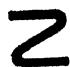
\includegraphics[keepaspectratio]{images/part002_c9cfa224.jpg}}

其中 \(f_x\) 是 \(G\) 到齐性空间 \(G/H_x\) 上的典范映射，\(g_x\) 是双射 \(s.H_x \to s.x\)（\(G/H_x\) 到 \(X\) 上的）；此外（第一章 § 3 第 4 目命题 6），\(g_x\) 是连续映射。但 \(g_x\) 未必是 \(G/H_x\) 到 \(X\) 上的一个同胚（习题 29）。若 \(g_x\) 对每个 \(x \in X\) 都是同胚，则称 \(X\)（拓扑群 \(G\) 的）为拓扑齐性空间；为此的充要条件是：对每个 \(x \in E\)，映射 \(s \to s.x\)（\(G\) 到 \(X\) 中的）是开的。

命题 15 设 X 是一个拓扑空间，拓扑群 G 连续且可迁地作用在它上面。为使 X 是（关于 G 的）拓扑齐性空间，只需对某一点 \(x_{0} \in X\)，映射 \(s \to s \cdot x_{0}\) 把 e 在 G 中的每个邻域变换为 \(x_{0}\) 在 X 中的一个邻域。

每个 \(x \in X\) 都可写作 \(x = t.x_0\)（对某个 \(t \in G\)）。若 \(V\) 是 \(e\) 的一个邻域，则 \(V.x = (Vt).x_0\) 是 \(x\) 的一个邻域，因为可以写 \((Vt).x_0 = t((t^{-1}Vt).x_0)\)，而断言由下列事实得出：\(t^{-1}Vt\) 是 \(e\) 在 \(G\) 中的一个邻域，且 \(y \to t.y\) 是 \(X\) 到其自身的一个同胚（第 4 目引理 1）。由此可得，若 \(U\) 是 \(G\) 的任一开子集且 \(x\) 是 \(X\) 的任一点，则 \(U.x\) 在 \(X\) 中是开的；因为若 \(t \in U\)，则 \(t^{-1}U\) 是 \(e\) 的一个邻域，因而 \((t^{-1}U).x\) 是 \(x\) 的一个邻域，且 \(t.((t^{-1}U).x) = U.x\) 是 \(t.x\) 的一个邻域。于是 \(U.x\) 在 \(X\) 中是开的，从而映射 \(s \to s.x\)（\(G\) 到 \(X\) 中的）是开的。证毕。

\subsection{商群}

命题 16 设 G 是一个拓扑群，H 是 G 的一个正规子群。则 G 的拓扑经 H 的商与 G/H 的群结构相容。

若 \(x \to \dot{x}\) 是 G 到 G/H 上的典范映射，则我们要证明的是：\((\dot{x}, \dot{y}) \to \dot{x}\dot{y}^{-1}\) 是 (G/H) \(\times\) (G/H) 到 G/H 中的一个连续映射。由于等价关系 \(x^{-1}y \in H\) 是开的（第 4 目引理 2），只需证明 \((x,y) \to \dot{x}\dot{y}^{-1}\) 是 G \(\times\) G 到 G/H 中的一个连续映射（第一章 § 5 第 3 目命题 8 的推论，以及 § 3 第 4 目命题 6）。但 \((x,y) \to \dot{x}\dot{y}^{-1}\) 是连续映射 \(x \to \dot{x}\) 与 \((x,y) \to xy^{-1}\) 的复合，因而是连续的。

在后续内容中，每当我们把拓扑群 G 的商群 G/H 作为拓扑群考虑时，除相反的情况有明确说明外，总应理解为 G/H 的拓扑是 G 的拓扑经 H 的商。

命题 17 设 \(\varphi\) 是拓扑群 \(\mathbf{G}\) 到商群 \(\mathrm{G / H}\) 上的典范映射。若 \(\mathfrak{B}\) 是 \(e\) 在 \(\mathbf{G}\) 中的一个基本邻域系，则 \(\varphi(\mathfrak{B})\) 是单位元 \(\varphi(e)\)（\(\mathrm{G / H}\) 的）的一个基本邻域系。

这是第一章 § 5 第 3 目命题 5 的一个特殊情形。

命题 13 与 14 对商群特别地给出：

命题 18 设 G 是一个拓扑群，H 是 G 的一个正规子群。

\begin{enumerate}
\def\labelenumi{\alph{enumi})}
\item
  商群 G/H 是 Hausdorff 的，当且仅当 H 在 G 中是闭的。
\item
  商群 G/H 是离散的，当且仅当 H 在 G 中是开的。
\end{enumerate}

若 G 是一个拓扑群，N 是 \(\{e\}\) 在 G 中的闭包，则 N 是 G 的一个闭正规子群（第 1 目命题 1），因而 G/N 是 Hausdorff 的；G/N 称为 G 的伴随 Hausdorff 群。

命题 19 若 H 是拓扑群 G 的一个离散正规子群，则 G/H 与 G 局部同构。

设 \(\mathbf{V}\) 是 \(e\) 在 \(\mathbf{G}\) 中的一个邻域，它不含 \(\mathbf{H}\) 中除 \(e\) 外的任何点，又设 \(\mathbf{W}\) 是 \(e\) 在 \(\mathbf{G}\) 中的一个对称开邻域，使得 \(\mathbf{W}^2 \subset \mathbf{V}\)。则 \(\mathbf{W}\) 上典范映射 \(\varphi\)（\(\mathbf{G}\) 到 \(\mathbf{G} / \mathbf{H}\) 上的）的限制是单射；因为若 \(x, y \in \mathbf{W}\) 且 \(\varphi(x) = \varphi(y)\)，则 \(x^{-1}y \in \mathbf{W}^2 \subset \mathbf{V}\) 且 \(x^{-1}y \in \mathbf{H}\)，于是 \(x = y\)。由命题 17 可知 \(\varphi\) 在 \(\mathbf{W}\) 上的限制是 \(\mathbf{W}\) 到 \(\varphi(\mathbf{W})\) 上的一个同胚；又因 \(\varphi(xy) = \varphi(x)\varphi(y)\) 对所有 \(x, y \in \mathbf{W}\) 成立，我们断定 \(\mathbf{G}\) 与 \(\mathbf{G} / \mathbf{H}\) 局部同构（§ 1 第 3 目命题 3）。

\subsection{商群的子群与商群}

设 G 是一个拓扑群，H 是 G 的一个正规子群，\(\varphi: G \to G/H\) 是典范映射。我们知道，若 \(A'\) 是 G/H 的一个子群，则 \(\varphi^{-1}(A')\) 是 G 的一个包含 H 的子群。反之，若 A 是 G 的一个子群，则 \(\varphi(A)\) 是 G/H 的一个子群；此外，存在商群 \(A/(A \cap H)\) 到 G/H 的子群 \(\varphi(A)\) 上的一个典范双射，以及 \(\varphi(A)\) 到商群 AH/H 上的一个典范双射，且这两个双射对群结构而言都是同构。

命题 20 设 A 是拓扑群 G 的一个子群，H 是 G 的一个正规子群，\(\varphi\) 表示 G 到 G/H 上的典范映射。则 \(\varphi(A)\) 到 AH/H 上的典范双射是拓扑群的一个同构。

这由前面的注记以及第 4 目命题 10 得出。

\pandocbounded{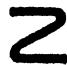
\includegraphics[keepaspectratio]{images/part002_0097f9c2.jpg}}

\(\mathbf{A}/(\mathbf{A} \cap \mathbf{H})\) 到 \(\varphi(\mathbf{A})\) 上的典范双射是连续同态，因为它是由 \(\varphi\) 在 \(\mathbf{A}\) 上的限制过渡到商而产生的；但一般地说，拓扑群 \(\mathbf{A}/(\mathbf{A} \cap \mathbf{H})\) 与 \(\mathbf{AH}/\mathbf{H}\) 不同构（参看 § 4 第 1 目命题 1 推论 3）。

* 例如，取 G 为实数的加法群 R，取 H 为整数群 Z，取 A 为一个无理数 θ 的整数倍组成的群 θZ。则 A∩H = \{0\}，因而 A/(A∩H) 是一个离散群，同构于 Z；另一方面，A + H 在 R 中稠密（我们将在第五章 § 1 第 1 目命题 1 中看到），于是 (A + H)/H——它与 A + H 局部同构（第 6 目命题 19）——不是离散群，从而不同构于 A/(A∩H)。*

尽管如此，我们有下面的命题：

命题 21 设 G 是一个拓扑群，\(G_{0}\) 是 G 的一个稠密子群，\(H_{0}\) 是 \(G_{0}\) 的一个正规子群，H 是 \(H_{0}\) 在 G 中的闭包，\(\varphi\) 是典范映射 \(G \rightarrow G/H\)。则典范双射 \(G_{0}/H_{0} \rightarrow \varphi(G_{0})\) 是拓扑群 \(G_{0}/H_{0}\) 到 G/H 的一个稠密子群上的一个同构。

由于 \(\mathbf{H}_0 = \mathbf{H} \cap \mathbf{G}_0\)，只需证明：若 \(\mathbf{U}_0\) 是 \(\mathbf{G}_0\) 的任一开子集，它关于关系 \(x^{-1}y \in \mathbf{H}_0\) 是饱和的，则 \(\mathbf{U}_0\) 是 \(\mathbf{G}_0\) 与 \(\mathbf{G}\) 的一个关于关系 \(x^{-1}y \in \mathbf{H}\) 饱和的开子集的交（第一章 § 3 第 6 目命题 10）。设 \(\mathbf{U}\) 是 \(\mathbf{G}\) 的一个使 \(\mathbf{U}_0 = \mathbf{U} \cap \mathbf{G}_0\) 的开子集。由于 \(\mathbf{U}_0 = \mathbf{U}_0\mathbf{H}_0\)，容易看出 \(\mathbf{U}_0 = \mathrm{UH}_0 \cap \mathbf{G}_0\)；但 \(\mathrm{UH}_0\) 在 \(\mathbf{G}\) 中是开的，故可设 \(\mathbf{U} = \mathrm{UH}_0\)。集合 \(\mathrm{UH}\) 在 \(\mathbf{G}\) 中是开的且关于关系 \(x^{-1}y \in \mathbf{H}\) 是饱和的；因此只要证明 \(\mathrm{UH} \cap \mathbf{G}_0 = \mathbf{U}_0\)，命题就证明了。现在，若 \(u \in \mathbf{U}\) 与 \(h \in \mathbf{H}\) 使 \(uh \in \mathbf{G}_0\)，则存在一个对称邻域 \(\mathbf{V}\)（\(e\) 在 \(\mathbf{G}\) 中的），使得 \(uv \subset U\)；由于 \(Vh\) 是 \(h\) 在 \(\mathbf{G}\) 中的一个邻域，存在 \(z \in V\) 使 \(zh \in \mathbf{H}_0\)。于是有 \(uz^{-1} \in U\)，且 \(uh = (uz^{-1})(zh)\)；因此 \(\mathrm{UH} \cap \mathbf{G}_0 \subset \mathrm{UH}_0\)。但 \(\mathrm{UH}_0 = U\)，于是 \(\mathrm{UH} \cap \mathbf{G}_0 \subset U \cap \mathbf{G}_0 = U_0\)。证毕。

设 G 是连续作用在拓扑空间 X 上的一个拓扑群，K 是 G 的一个正规子群，它含于 X 的每一点的稳定子群中。对每个 \(x \in X\)，关系 \(s \equiv t \pmod{K}\) 因而蕴含 s.x = t.x，并且过渡到商，我们定义一个 G/K 到 X 中的映射 \(\dot{s} \to \dot{s}.x\)。立即可验证，关于外法则 \((\dot{s}, x) \to \dot{s}.x\)，X 以 G/K 为算子群。此外，G/K 关于这个法则连续作用在 X 上；因为 X 上的相等关系与 G 上的关系 \(s \equiv t \pmod{K}\) 都是开的等价关系，于是结论由映射

\[
(s, x) \rightarrow \dot {s}. x = s. x
\]

（\(\mathbf{G} \times \mathbf{X}\) 到 \(\mathbf{X}\) 中的）的连续性得出（第一章 § 5 第 3 目命题 8 的推论，以及 § 3 第 4 目命题 6）。

现设 G 是连续作用在拓扑空间 X 上的一个拓扑群，H 是 G 的任一正规子群；则 H 连续作用在 X 上。设 S 是 H 在 X 上定义的等价关系；则 S 是开的（第 4 目引理 2）。关系 S 与群 G 相容（第 4 目）；因为若 \(y \equiv x \pmod{S}\)，则存在 \(t \in H\) 使 y = t.x；于是对所有 \(s \in G\) 有 \(s.y = (sts^{-1}) \cdot s.x\)，且由于 H 在 G 中正规，有 \(sts^{-1} \in H\)；从而 \(s.y \equiv s.x \pmod{S}\)。若 \(\psi\) 是 X 到 X/S 上的典范映射，则群 G 关于外法则

\[
(s, \psi (x)) \rightarrow \psi (s. x)
\]

（第 4 目命题 11）。此外，群 H 含于 X/S 的每一点的稳定子群中；如我们上面所见，G/H 关于外法则 \((s, \psi(x)) \to \psi(s.x)\) 连续作用在 X/S = X/H 上。若 R 表示 G 在 X 上定义的等价关系，则关系 S 蕴含 R，且 X/S 上的等价关系 R/S 是由群 G/H 定义的。因此（第一章 § 3 第 4 目命题 7）：

命题 22 设 G 是连续作用在拓扑空间 X 上的一个拓扑群，H 是 G 的一个正规子群。则 X/G 到 (X/H)/(G/H) 上的典范双射是一个同胚。

推论 设 G 是一个拓扑群，H 是 G 的一个正规子群，K 是 G 的一个包含 H 的正规子群。则 G/K 到 (G/H)/(K/H) 上的典范双射是拓扑群的一个同构。

我们已知道这个双射是群的一个同构，而命题 22（应用于在 G 的右边作用的群 K）表明它是一个同胚。

\subsection{连续同态与严格态射}

命题 23 同态 \(f\)（拓扑群 \(\mathbf{G}\) 到拓扑群 \(\mathbf{G}'\) 中的）在 \(\mathbf{G}\) 上连续，当且仅当它在 \(\mathbf{G}\) 的一点处连续。

设 \(f\) 在一点 \(a \in \mathbf{G}\) 处连续；则若 \(\mathbf{V}'\) 是 \(f(a)\) 的任一邻域，\(\mathbf{V} = f^{-1}(\mathbf{V}')\) 是 \(a\) 的一个邻域。因而若 \(x\) 是 \(\mathbf{G}\) 的任一点，我们有

\[
f (x a ^ {- 1} \mathrm{V}) = f (x) [ f (a) ] ^ {- 1} f (\mathrm{V}) \subset f (x) [ f (a) ] ^ {- 1} \mathrm{V} ^ {\prime},
\]

因而 \(f\) 在 \(x\) 处连续。

拓扑群 G 到拓扑群 \(G'\) 中的连续同态也称为 G 到 \(G'\) 中的（对拓扑群结构而言的）态射。

设 \(f\) 是拓扑群 \(G\) 到拓扑群 \(G'\) 中的一个连续同态；原像 \(H = f^{-1}(e')\)——这里 \(e'\) 是 \(G'\) 的单位元——是 \(G\) 的一个正规子群，且 \(f(G)\) 是 \(G'\) 的一个子群。考虑典范分解 \(f = \psi \circ \overline{f} \circ \varphi\)，其中 \(\varphi\) 是典范映射 \(G \to G/H\)，\(\psi\) 是典范单射 \(f(G) \to G'\)，最后 \(\overline{f}\) 是商群 \(G/H\) 到子群 \(f(G)\) 上的一个连续双射同态（第一章 § 3 第 5 目）；称 \(\overline{f}\) 为伴随于 \(f\) 的双射同态。一般地说，\(f\) 不是拓扑群的一个同构。

例如，设 \(G'\) 是一个非离散拓扑群，G 是把离散拓扑赋予 \(G'\) 所得的拓扑群；则 G 到 \(G'\) 中的恒等映射是连续双射同态，但不是双连续的。

定义 1 拓扑群 G 到拓扑群 \(\mathbf{G}'\) 中的连续同态称为 G 到 \(\mathbf{G}'\) 中的严格态射，如果双射同态 \(\overline{f}\)（从 \(\mathbf{G}/f^{-1}(e')\) 到 \(f(\mathbf{G})\) 上的，伴随于 \(f\)）是拓扑群的一个同构（换言之，如果 \(\overline{f}\) 是双连续的）。

因此拓扑群 G 到拓扑群 \(G'\) 上的一个同构是 G 到 \(G'\) 上的一个双射严格态射。

命题 24 设 \(f\) 是拓扑群 \(G\) 到拓扑群 \(G'\) 中的一个连续同态。则下列三个命题等价：a) \(f\) 是严格态射。

\begin{enumerate}
\def\labelenumi{\alph{enumi})}
\setcounter{enumi}{1}
\item
  在 \(f\) 下，\(\mathbf{G}\) 中每个开集的像是 \(f(\mathbf{G})\) 中的一个开集。
\item
  在 \(f\) 下，\(G\) 的单位元的每个邻域的像是 \(G'\) 的单位元的一个邻域。
\end{enumerate}

鉴于第 4 目引理 2，a) 与 b) 的等价性由定义立即得出（第一章 § 5 第 3 目命题 5）。b) 与 c) 的等价性是第 5 目命题 15 的一个特殊情形，只要注意到 G 连续作用在 \(f(\mathbf{G})\) 上，其外法则是 \((s, f(t)) \to f(st)\)。

注。1) 由命题 24 的条件 b) 可得，拓扑群到离散群中的每个连续同态都是严格态射。

若 G 是紧的且 \(f(\mathbf{G})\) 是 Hausdorff 的，则伴随于 f 的双射同态 \(\overline{f}\) 是双连续的（第一章 § 10 第 2 目定理 1 推论 2，以及第 1 目命题 5 推论 4）。因此紧群到 Hausdorff 群中的每个连续同态都是严格态射。

\pandocbounded{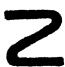
\includegraphics[keepaspectratio]{images/part002_802da4a7.jpg}}

\begin{enumerate}
\def\labelenumi{\arabic{enumi})}
\setcounter{enumi}{1}
\item
  设 \(f\) 是 \(G\) 到 \(G'\) 中的一个严格态射，\(g\) 是 \(G'\) 到 \(G''\) 中的一个严格态射。若 \(f\) 是满射或 \(g\) 是单射，则由命题 24 立即得出 \(g \circ f\) 是 \(G\) 到 \(G''\) 中的一个严格态射。但如果前面两个条件没有一个满足，这个结论就未必成立，即使 \(f\) 是单射且 \(g\) 是满射（习题 19）。
\item
  设 \(f\) 是拓扑群 \(G\) 到拓扑群 \(G'\) 中的一个连续同态，\(H\) 是 \(G\) 的一个正规子群。\(f\) 诱导一个同态 \(g\)（群 \(G / H\) 到商群 \(f(G) / f(H)\) 上的）。这个同态 \(g\) 是连续的。此外，若 \(f\) 是 \(G\) 到 \(G'\) 中的一个严格态射，则 \(g\) 是 \(G / H\) 到 \(f(G) / f(H)\) 上的一个严格态射；因为若 \(U\) 在 \(G / H\) 中是开的，且以 \(\varphi\)（相应地 \(\varphi'\)）表示 \(G\) 到 \(G / H\) 上{[}相应地 \(f(G)\) 到 \(f(G) / f(H)\) 上{]}的典范映射，则有 \(g(u) = \varphi'(f(\varphi^{-1}(u)))\)，而由于 \(\varphi^{-1}(u)\) 在 \(G\) 中是开的，可知 \(g(u)\) 在 \(f(G) / f(H)\) 中是开的，这就证明了我们的断言。
\end{enumerate}

\subsection{拓扑群的积}

设 \((\mathbf{G}_i)_{i\in I}\) 是一个拓扑群族。则我们可以在积集上定义一个群结构

\[
\mathbf {G} = \prod_ {i \in I} \mathbf {G} _ {i}
\]

（诸 \(\mathbf{G}_i\) 的群结构的积），办法是定义 \((x_i) \cdot (y_i) = (x_i y_i)\)。若 \(e_i\) 是 \(\mathbf{G}_i\) 的单位元，则 \(e = (e_i)\) 是 \(\mathbf{G}\) 的单位元，且有 \((x_i)^{-1} = (x_i^{-1})\)。诸 \(\mathbf{G}_i\) 的拓扑的积拓扑（第一章 § 2 第 3 目）与这个群结构相容。因为映射 \(((x_i), (y_i)) \to (x_i y_i^{-1})\)（\(\mathbf{G} \times \mathbf{G}\) 到 \(\mathbf{G}\) 中的）是下列映射的复合：映射 \(((x_i, y_i)) \to (x_i y_i^{-1})\)（从

\[
\prod_ {i \in I} G _ {i} \times G _ {i} \text {   into   } G,
\]

）以及典范映射 \(((x_{i}), (y_{i})) \to ((x_{i}, y_{i}))\)（从

\[
\mathbf {G} \times \mathbf {G} \quad \text { onto } \quad \prod_ {i \in \mathbf {I}} (\mathbf {G} _ {i} \times \mathbf {G} _ {i});
\]

）；而这两个映射都是连续的（第一章 § 4 第 1 目命题 1 的推论 1，以及命题 2）。

定义 2 把积集

\[
\mathbf {G} = \prod_ {i \in \mathbf {I}} \mathbf {G} _ {i}
\]

赋予诸 \(G_{i}\) 的群结构的积这个群结构与诸 \(G_{i}\) 的拓扑的积这个拓扑所得的拓扑群，称为诸拓扑群 \(G_{i}\) 的积。

若 \((\mathbf{J}_{\kappa})_{\kappa \in \mathbb{K}}\) 是 I 的一个划分，则 G 同构于诸拓扑群 \(\prod_{i \in J_{\kappa}} G_{i}\) 的积（积的结合性）。

若 \(\mathbf{H}_{i}\) 是 \(\mathbf{G}_{i}\) 的一个子群，则诸拓扑群 \(\mathbf{H}_{i}\) 的积同构于子群 \(\prod_{i} \mathbf{H}_{i}\)（\(\prod_{i} \mathbf{G}_{i}\) 的）。特别地，若 \(J\) 是 \(I\) 的任一子集，且 \(J' = C_{J}\)，则拓扑群 \(\prod_{i \in J} \mathbf{G}_{i}\) 同构于正规子群 \(\mathbf{G}_{J}' = (\prod_{i \in J} \mathbf{G}_{i}) \times (\prod_{i' \notin J} \{e_{i'}\})\)（\(\mathbf{G}\) 的）。由于每个开集的投影是开集，投影 \(\mathbf{pr}_{J}\)（\(\mathbf{G}\) 到 \(\prod_{i \in J} \mathbf{G}_{i}\) 上的）是严格态射，因而商群 \(\mathbf{G} / \mathbf{G}_{J}'\) 同构于 \(\mathbf{G}_{J'}'\)；\(\mathbf{G}\) 同构于积 \(\mathbf{G}_{J}' \times (\mathbf{G} / \mathbf{G}_{J}')\)。

命题 25 设 \((\mathbf{G}_{i})_{i\in I}\) 是一个拓扑群族，H 是 \(\mathbf{G} = \prod_{i\in I}\mathbf{G}_i\) 的由所有这样的 \(x = (x_{i})\) 组成的正规子群：诸 \(x_{i}\) 除有限个指标外都等于单位元 \(e_i\)（\(\mathbf{G}_i\) 的）。则子群 H 在 G 中稠密。

这是第一章 § 4 第 3 目命题 8 的一个特殊情形。

设 \((\mathbf{X}_i)_{i \in I}\) 是一个拓扑空间族，且对每个 \(i \in I\)，设 \(\mathbf{G}_i\) 是连续作用在 \(\mathbf{X}_i\) 上的一个拓扑群。显然，积群 \(\mathbf{G} = \prod_{i \in I} \mathbf{G}_i\) 这时依照法则连续作用在积空间 \(\mathbf{X} = \prod_{i \in I} \mathbf{X}_i\) 上

\[
\left(\left(s _ {i}\right), \left(x _ {i}\right)\right)\rightarrow \left(s _ {i}. x _ {i}\right)
\]

（第一章 § 4 第 1 目命题 1 推论 1，以及命题 2）。此外，X 的点 \(x = (x_{i})\) 在 G 下的轨道是诸 \(x_{i}\) 的轨道（关于诸群 \(G_{i}\) 的）的积。设 \(\varphi_{i}\) 是 \(X_{i}\) 到 \(X_{i}/G_{i}\) 上的典范映射，\(\varphi = (\varphi_{i})\) 是 X 到 \(\prod_{i\in I}(X_{i}/G_{i})\) 上的积映射；则前面的注记表明，典范地伴随于 \(\varphi\) 的双射把轨道空间 X/G 映为 \(\prod_{i\in I}(X_{i}/G_{i})\)。此外：

命题 26 X/G 到 \(\prod_{i\in I}(\mathbf{X}_i / \mathbf{G}_i)\) 上的双射（典范地伴随于 \((\varphi_i)\) 的）是一个同胚。

因为诸 \(\varphi_{i}\) 是满射且开的，可知 \(\varphi = (\varphi_{i})\) 是一个开映射（第一章 § 5 第 3 目命题 8 的推论）。

推论 设 \((\mathbf{G}_{i})_{i\in I}\) 是一个拓扑群族，且对每个 \(i\in I\)，设 \(\mathbf{H}_i\) 是 \(\mathbf{G}_i\) 的一个正规子群；以 \(\varphi_i\) 表示 \(\mathbf{G}_i\) 到 \(\mathbf{G}_i / \mathbf{H}_i\) 上的典范映射。设 \(\mathbf{G} = \prod_{i\in I}\mathbf{G}_i\)，\(\mathbf{H} = \prod_{i\in I}\mathbf{H}_i\)。则 \(\mathbf{G} / \mathbf{H}\) 到 \(\prod_{i\in I}(\mathbf{G}_i / \mathbf{H}_i)\) 上的、伴随于连续同态 \((x_i)\to (\varphi_i(x_i))\) 的双射同态是拓扑群的一个同构。

因为这个同态是群结构的一个同构。

注。若 G 是一个交换拓扑群，以加法记，则映射 \((x,y)\to x+y\)（\(G\times G\) 到 G 上的）是一个严格态射。因为由于 \((x+x')+(y+y')=(x+y)+(x'+y')\)，它是 \(G\times G\) 到 G 上的一个同态；它也是连续的，且邻域 \(V\times V\)（\(G\times G\) 中原点的）在这个映射下的像是 G 中原点的邻域 \(V+V\)。

\subsection{半直积}

设 L、N 是群 G 的两个子群，使得 LN = NL；则 LN 是 G 的一个子群，因为

\[
(\mathrm{LN}) (\mathrm{LN}) ^ {- 1} = \mathrm{LNN} ^ {- 1} \mathrm{L} ^ {- 1} = \mathrm{LNL} = \mathrm{LLN} = \mathrm{LN}
\]

此外，映射 \(\varphi: (x, y) \to xy\)（\(N \times L\) 到 \(G\) 中的）是单射，当且仅当 \(N \cap L = \{e\}\)。因为显然若 \(\varphi\) 是单射，则 \(N \cap L = \{e\}\)；反之，关系 \(x' y' = xy\)（其中 \(x, x' \in N\)，\(y, y' \in L\)）蕴含 \(x^{-1}x' = yy'^{-1} \in N \cap L\)；因此若 \(N \cap L = \{e\}\)，则 \(\varphi\) 是单射。于是 \(\varphi\) 是双射，当且仅当 \(LN = G\) 且 \(N \cap L = \{e\}\)。

若 N 是 G 的一个正规子群（或更一般地，在 G 的某个包含 \(N \cup L\) 的子群中是正规的），则条件 LN = NL 自动满足。此外，对每个 \(y \in L\)，映射 \(\sigma_{y}: x \to yxy^{-1}\) 是群 N 的一个自同构，且对 L 的任意两个元素 u、v，我们有

\[
\sigma_ {u v} = \sigma_ {u} \circ \sigma_ {v};\tag{1}
\]

而且对任意 \(x, x'\)（\(\mathbf{N}\) 中的）与任意 \(y, y'\)（\(\mathbf{L}\) 中的），我们还有

\[
(x y) (x ^ {\prime} y ^ {\prime}) = (x \sigma_ {y} (x ^ {\prime})) (y y ^ {\prime}).\tag{2}
\]

反过来：

命题 27 设 N 与 L 是两个群，\(e'\) 与 \(e''\) 是它们各自的单位元。设给定了同态 \(y \to \sigma_y\)（L 到 N 的自同构群 \(\Gamma\) 中的）。则：

\begin{enumerate}
\def\labelenumi{\arabic{enumi})}
\tightlist
\item
  在积集 \(\mathbf{S} = \mathbf{N} \times \mathbf{L}\) 上，内合成法则
\end{enumerate}

\[
(x, y) (x ^ {\prime}, y ^ {\prime}) = (x \sigma_ {y} (x ^ {\prime}), y y ^ {\prime})\tag{3}
\]

定义了一个群结构，对这个结构，\(j_1: x \to (x, e'')\) 是 \(N\) 到 \(S\) 的一个正规子群上的同构，\(j_2: y \to (e', y)\) 是 \(L\) 到 \(S\) 的一个子群上的同构，而 \(\mathrm{pr}_2: S \to L\) 是一个满射同态，其核是 \(j_1(N)\)，并且使得 \(\mathrm{pr}_2 \circ j_2\) 是 \(L\) 的恒等自同构。

\begin{enumerate}
\def\labelenumi{\arabic{enumi})}
\setcounter{enumi}{1}
\tightlist
\item
  设 \(f: \mathbf{N} \to \mathbf{G}\)，\(g: \mathbf{L} \to \mathbf{G}\) 是到一个群 \(\mathbf{G}\) 中的两个同态，使得
\end{enumerate}

\[
f (\sigma_ {y} (x)) = g (y) f (x) g (y ^ {- 1})\tag{4}
\]

对所有 \(x \in \mathbb{N}\) 与所有 \(y \in \mathbb{L}\) 成立。则存在唯一的同态 \(h: \mathbb{S} \to \mathbb{G}\)，使得 \(f = h \circ j_1\) 且 \(g = h \circ j_2\)。

若 \(x, x', x''\) 是 N 的元素，\(y, y', y''\) 是 L 的元素，则

并且

\[
\begin{array}{r l} ((x, y) (x ^ {\prime}, y ^ {\prime})) (x ^ {\prime \prime}, y ^ {\prime \prime}) & = (x \sigma_ {y} (x ^ {\prime}), y y ^ {\prime}) (x ^ {\prime \prime}, y ^ {\prime \prime}) \\ & = (x \sigma_ {y} (x ^ {\prime}) \sigma_ {y y ^ {\prime}} (x ^ {\prime \prime}), y y ^ {\prime} y ^ {\prime \prime}) \\ (x, y) ((x ^ {\prime}, y ^ {\prime}) (x ^ {\prime \prime}, y ^ {\prime \prime})) & = (x, y) (x ^ {\prime} \sigma_ {y ^ {\prime}} (x ^ {\prime \prime}), y ^ {\prime} y ^ {\prime \prime}) \\ & = (x \sigma_ {y} (x ^ {\prime} \sigma_ {y ^ {\prime}} (x ^ {\prime \prime})), y y ^ {\prime} y ^ {\prime \prime}) \end{array}
\]

因而法则 (3) 的结合律由下列事实得出：\(y \to \sigma_{y}\) 是 L 到 \(\Gamma\) 中的一个同态，且 \(\sigma_{y}\) 是 N 的一个自同构。显然 \((e', e'')\) 是 (3) 的单位元，最后

\[
(x, y) \left(\sigma_ {y ^ {- 1}} (x ^ {- 1}), y ^ {- 1}\right) = \left(\sigma_ {y ^ {- 1}} (x ^ {- 1}), y ^ {- 1}\right) (x, y) = \left(e ^ {\prime}, e ^ {\prime \prime}\right)
\]

于是 \((x, y)\) 在 S 中有一个逆元。1) 的其余断言是清楚的。另一方面，由于 \((x, y) = (x, e'') (e', y)\)，满足 2) 的条件的同态 \(h\) 必然满足

\[
h (x, y) = f (x) g (y),
\]

因而若它存在则是唯一的；此外，由 (4) 立即得出

\[
f \left(x \sigma_ {y} (x ^ {\prime})\right) g (y y ^ {\prime}) = f (x) g (y) f (x ^ {\prime}) g (y ^ {- 1}) g (y) g (y ^ {\prime}) = f (x) g (y) f (x ^ {\prime}) g (y ^ {\prime})
\]

这表明 \((x, y) \to f(x)g(y)\) 确是 S 到 G 中的、满足 2) 的条件的一个同态。

推论 命题 27 的 2) 中定义的同态 \(h\) 是单射，当且仅当 \(f\) 与 \(g\) 都是单射且 \(f(\mathbf{N}) \cap g(\mathbf{L}) = \{e\}\)；而 \(h\) 是满射，当且仅当 \(f(\mathbf{N})g(\mathbf{L}) = \mathbf{G}\)。

由于 \(h(x, y) = f(x)g(y)\)，第二个断言是显然的；此外由 (4) 可得 \(f(\mathbf{N})g(\mathbf{L}) = g(\mathbf{L})f(\mathbf{N})\)，而第一个断言由本小节开头的注记得出。

命题 27 中定义的群 S 称为 N 与 L 的外半直积（关于 \(\sigma\) 的）；我们通常把 N（相应地 L）等同于 S 的正规子群 \(j_{1}(N)\){[}相应地子群 \(j_{2}(L)\){]}。若 \(\sigma_{y}\) 是 \(\Gamma\) 的单位元（对所有 \(y \in L\)），我们就重新得到两个群的积的通常概念。

现设 G 是一个群，L 与 N 是 G 的两个子群，使得 LN = NL 且 N 在 NL 中正规，于是对每个 \(y \in L\)，\(\sigma_{y} : x \to yxy^{-1}\) 是 N 的一个自同构，且 \(y \to \sigma_{y}\) 是 L 到 N 的自同构群 \(\Gamma\) 中的一个同态。于是由命题 27 可得：若 S 是 N 与 L 的外半直积（关于 \(\sigma\) 的），则 \(h : (x, y) \to xy\) 是 S 到 G 中的一个同态。h 是双射，当且仅当我们有 \(N \cap L = \{e\}\) 且 NL = G（命题 27 的推论）；这时称 G 为其正规子群 N 与其子群 L 的半直积，且我们常借助于 h 把 G 等同于 S。

命题 28 设 L、N 是两个拓扑群，\(y \to \sigma_y\) 是 L 到 N 的（非拓扑的）群结构的自同构群 \(\Gamma\) 中的一个同态；并设映射 \((x, y) \to \sigma_y(x)\)（\(N \times L\) 到 N 中的）是连续的。则：

\begin{enumerate}
\def\labelenumi{\arabic{enumi})}
\item
  在 N 与 L 的外半直积 S（关于 \(\sigma\) 的）上，N 与 L 的拓扑的积与群结构相容；典范单射 \(j_{1}: \mathrm{N} \to \mathrm{S}\) 与 \(j_{2}: \mathrm{L} \to \mathrm{S}\) 分别是拓扑群 N 与 L 到 S 的子群 \(j_{1}(\mathrm{N})\) 与 \(j_{2}(\mathrm{L})\) 上的同构，而 \(pr_{2}\) 是 S 到 L 上的一个严格态射。
\item
  设 \(f: \mathbf{N} \to \mathbf{G}\) 与 \(g: \mathbf{L} \to \mathbf{G}\) 是到一个拓扑群 \(\mathbf{G}\) 中的两个连续同态，满足 (4)；则同态
\end{enumerate}

\[
(x, y) \rightarrow f (x) g (y)
\]

（S 到 G 中的）是连续的。

这是定义以及积拓扑的性质的一个直接推论。

这样定义的拓扑群 S 称为 N 与 L 的拓扑外半直积（关于 \(\sigma\) 的）；注意，加于 \(\sigma\) 的条件蕴含 L 依照外法则 \((x, y) \to \sigma_{y}(x)\) 在 N 的左边连续作用{[}第 4 目{]}。

现设 G 是一个拓扑群，N 与 L 是 G 的两个子群，使得 G 作为非拓扑群是 N 与 L 的半直积；则显然映射 \((x, y) \to \sigma_{y}(x)\) 在 \(N \times L\) 上连续，且典范双射同态

\[
h: (x, y) \rightarrow x y
\]

（S 到 G 上的）是连续的。但这个同态未必是双连续的；当它双连续时，称 G 为 N 与 L 的拓扑半直积。为此的充要条件是：若 \(p: G \to N\) 与 \(q: G \to L\) 是使 \(z \in G\) 对应于唯一的元素 \(p(z) \in N\) 与 \(q(z) \in L\)（满足 \(z = p(z)q(z)\)）的映射，则映射 p、q 之一是连续的（这时两者都是连续的）。这等同于说，典范映射 \(G \to G/N\) 在 L 上的限制是拓扑群 L 到拓扑群 G/N 上的一个同构。

\section{群上的一致结构}

\subsection{拓扑群的右一致结构与左一致结构}

在拓扑群 G 中，我们可以察觉到按下述方式定义“充分近的点”这个概念、从而定义一个一致结构的可能性：若 x 与 y 是 G 的任意两点，我们对这两点施加把其中之一（比如说 x）送到单位元 e 的平移；x 与 y 的“接近程度”这时在某种意义上由 y 被送入的 e 的邻域 V 来衡量。这个平移——它在于把 x 与 y 都乘以 \(x^{-1}\)——可以在右边或在左边进行，而我们将看到，在这两种情形我们都确实得到 G 上的一个与 G 的拓扑相容的一致结构。取平移在右边进行的情形；于是对 e 的每个邻域 V 对应有集 \(V_{d}\)，即偶 \((x, y) \in \mathbf{G} \times \mathbf{G}\)（满足 \(yx^{-1} \in V\) 的）组成的集。设 \(G_{d}\) 是诸集 \(V_{d}\) 的族，其中 V 跑遍 e 的邻域滤子 B。则 \(G_{d}\) 是一个基本一致邻域系（第二章 § 1 第 1 目）。因为由于 \(e \in V\)，对角线 \(\Delta\)（\(G \times G\) 的）含于 \(V_{d}\)（对每个 \(V \in B\)），于是 \(G_{d}\) 是一个滤子基且满足公理 \((\mathrm{U}_{\mathrm{I}}^{\prime})\)；由于关系 \(yx^{-1} \in V\) 与 \(xy^{-1} \in V^{-1}\) 等价，我们有 \(\mathbf{V}_{d}^{-1} = (\mathbf{V}^{-1})_{d}\)。

于是 \(\mathbf{V}_{d}^{-1}\in \mathfrak{G}_d\)（由 \((\mathrm{GV}_{\mathrm{II}})\)），从而 \((\mathrm{U}_{\mathrm{II}}^{\prime})\) 满足；最后，关系 \(zx^{-1}\in \mathrm{V}\) 与 \(yz^{-1}\in \mathrm{V}\) 蕴含 \(yx^{-1}\in \mathrm{V.V}\)；于是 \(\mathbf{V}_d\circ \mathbf{V}_d\) 含于 \((\mathrm{V.V})_d\)，而 \((\mathrm{GV}_{\mathrm{I}})\) 表明 \(\mathfrak{G}_d\) 满足 \((\mathrm{U}_{\mathrm{III}}^{\prime})\)。

由 \(\mathfrak{G}_d\) 定义的一致结构与 \(\mathbf{G}\) 的拓扑相容，因为关系 \(y \in \mathrm{V}_d(x)\) 与 \(y \in \mathrm{V}.x\) 依定义等价；换言之，\(\mathrm{V}_d(x) = \mathrm{V}.x\)。

当平移在左边进行时，论证是类似的，因此我们可以给出下面的定义：

定义 1 拓扑群 G 的右（相应地，左）一致结构是指这样的一致结构：使单位元 e 的每个邻域 V 对应于集 \(V_{d}\)（相应地 \(V_{s}\)），它由这样的偶 \((x, y)\) 组成：使得 \(y x^{-1} \in V\)（相应地 \(x^{-1} y \in V\)），就得到它的一个基本一致邻域系。

若 V 跑遍 e 的一个基本邻域系，则诸集 \(V_{d}\)（相应地 \(V_{s}\)）构成右（相应地，左）一致结构的一个基本一致邻域系。

一致空间拓扑的每个命题对应着群拓扑的一个命题；翻译依照定义 1 及公式 \(\mathrm{V}_{d}(x)=\mathrm{V}.x,\quad\mathrm{V}_{d}(\mathrm{A})=\mathrm{V}.\mathrm{A},\quad\mathrm{V}_{s}(x)=x.\mathrm{V},\quad\mathrm{V}_{s}(\mathrm{A})=\mathrm{A}.\mathrm{V}\) 进行，这些公式是定义的直接推论。例如，若 A 是 G 的任一非空子集，则我们有（第二章 § 1 第 2 目命题 2 推论 1）

\[
\overline {{{\mathrm{A}}}} = \bigcap_ {\mathbf {V} \in \mathfrak {B}} \mathrm{V}. \mathrm{A} = \bigcap_ {\mathbf {V} \in \mathfrak {B}} \mathrm{A}. \mathrm{V}.\tag{1}
\]

又如（第二章 § 1 第 2 目命题 2 推论 3），每个 Hausdorff 群都是正则的。

拓扑群的右一致结构与左一致结构一般是不同的（见习题 4）。显然，若群是交换的，它们一致，因为这时 \(\mathbf{V}_d = \mathbf{V}_s\)；若群是紧的，它们也一致（第二章 § 4 第 1 目定理 1）。

一般地，我们以 \(G_{s}\)（相应地 \(G_{d}\)）表示把左（相应地，右）一致结构赋予集 G 所得的一致空间。

命题 1 左平移与右平移是右一致结构到其自身的同构。

至于右平移，结果是清楚的，因为关系 \(yx^{-1} \in V\) 等价于 \((ya)(xa)^{-1} \in V\){[}换言之，映射 \((x, y) \to (xa, ya)\) 使 \(V_d\) 不变{]}。至于左平移，结果由 \((\mathrm{GV}_{\mathrm{III}})\) 得出；因为 \(yx^{-1} \in V\) 当且仅当 \((ay)(ax)^{-1} \in aVa^{-1}\)；于是 \(x \to ax\) 在 \(G_{d}\) 上一致连续。

类似地，右平移与左平移是左一致结构到其自身的同构。

因而 G 的每个内自同构 \(x \rightarrow axa^{-1}\) 对 G 的群结构、对 G 的拓扑以及对 G 的两个一致结构都是自同构。

命题 2 对称映射 \(x \to x^{-1}\) 是右一致结构到左一致结构上的一个同构。

这是定义 1 的一个直接推论。

\pandocbounded{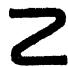
\includegraphics[keepaspectratio]{images/part002_77aeac5d.jpg}}

读者应当警惕，不要以为映射 \((x, y) \to xy\)（一致空间 \(G_{d} \times G_{d}\) 到一致空间 \(G_{d}\) 中的）一般是一致连续的。类似地，对称映射 \(x \to x^{-1}\)（视为 \(G_{d}\) 到 \(G_{d}\) 上的映射时）一般不是一致连续的（见习题 3 与 4）。

命题 3 每个连续同态 \(f\)（拓扑群 \(G\) 到拓扑群 \(G'\) 中的），视为 \(G_d\) 到 \(G_d'\) 中（或 \(G_s\) 到 \(G_s'\) 中）的映射时，是一致连续的。

因为若 \(V'\) 是 \(G'\) 中单位元的一个邻域，且 \(\mathbf{V} = f^{-1}(\mathbf{V}')\)，则关系 \(yx^{-1} \in V\) 蕴含

\[
f (y) (f (x)) ^ {- 1} = f (y x ^ {- 1}) \in V ^ {\prime}.
\]

\subsection{子群、商群与积群上的一致结构}

若 H 是拓扑群 G 的一个子群，则 G 的右一致结构在 H 上诱导的一致结构正是拓扑群 H 的右一致结构。

若 H 是 G 的一个正规子群，且 \(\varphi\) 是 G 到 G/H 上的典范映射，则使 G 中单位元的每个邻域 V 对应于 G/H 的所有偶 \((\dot{x},\dot{y})\)（满足 \(\dot{x}\dot{y}^{-1}\in \varphi (\mathrm{V})\) 的）组成的集，就得到商群 G/H 的右一致结构的一个基本一致邻域系（§ 2 第 6 目命题 17）。这个条件意味着至少有一点 \(x\in \dot{x}\) 且至少有一点 \(y\in \dot{y}\) 使 \(yx^{-1}\in V\){[}即使 \((x,y)\in V_d]\)。特别地，若 N 是 G 的子集 \(\{e\}\) 的闭包，则 G/N 上的右一致结构同构于伴随于 G 上右一致结构的 Hausdorff 一致结构（参看第二章 § 3 第 8 目）。

最后，在拓扑群族 \((\mathbf{G}_{i})\) 的积上，右一致结构是诸 \(G_{i}\) 的右一致结构的积（参看第二章 § 2 第 6 目）。

对左一致结构有类似的结果。

积群 \(\prod_{i\in I}G_i\) 上的左一致结构与右一致结构相同，当且仅当每个因子 \(G_{i}\) 上的左一致结构与右一致结构一致。如果某些 \(G_{i}\) 是交换的而其余的是紧的，情形总如此。

\subsection{完备群}

定义 2 拓扑群称为完备的，如果它的左一致结构与右一致结构都是完备空间的结构。

由第 1 目命题 2，为使一个群是完备的，只需它的两个一致结构之一是完备空间的结构。G 完备当且仅当它的伴随 Hausdorff 群（§ 2 第 6 目）完备。

完备群的每个闭子群是完备的（第二章 § 3 第 4 目命题 8）。完备群的每个积是完备的（第二章 § 3 第 5 目命题 10）。

\pandocbounded{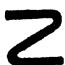
\includegraphics[keepaspectratio]{images/part002_8d186292.jpg}}

另一方面，若 G 是一个完备群且 H 是 G 的一个闭正规子群，则商群 G/H 未必完备（但参看第九章 § 3 第 1 目命题 4）。

命题 4 若在拓扑群 G 中存在 e 的一个邻域 V，它关于右一致结构或左一致结构之一是完备的，则 G 是完备的。

例如设 V 关于右一致结构是完备的，并设 F 是 \(G_{d}\) 上的一个 Cauchy 滤子；则 F 含有一个 \(V_{d}\)-小集 M，且若 \(x_{1} \in M\)，我们因而有 \(M \subset Vx_{1}\)。于是 F 在完备子空间 \(Vx_{1}\)（\(G_{d}\) 的）上的迹是一个 Cauchy 滤子，它收敛于一点 \(x_{0}\)；由于 \(x_{0}\) 是 F 的聚点，它是 F 的极限（第二章 § 3 第 2 目命题 5 推论 2）。

推论 1 局部紧群是完备的。

因为每个紧空间关于它的唯一的一致结构是完备的（第二章 § 4 第 1 目定理 1）。

推论 2 Hausdorff 拓扑群 G 的每个局部紧子群在 G 中是闭的。

因为 Hausdorff 一致空间的每个完备子空间是闭的（第二章 § 3 第 4 目命题 8）。

命题 5 设 \(G_{1}\) 是一个拓扑群，\(G_{2}\) 是一个完备的 Hausdorff 拓扑群，\(H_{1}\)（相应地 \(H_{2}\)）是 \(G_{1}\)（相应地 \(G_{2}\)）的一个稠密子群。则 \(H_{1}\) 到 \(H_{2}\) 中的每个连续同态 u 可以唯一地延拓为一个连续同态 \(\overline{u}\)（\(G_{1}\) 到 \(G_{2}\) 中的）。此外，若 \(G_{1}\) 是 Hausdorff 的且完备的，且 u 是 \(H_{1}\) 到 \(H_{2}\) 上的一个同构，则 \(\overline{u}\) 是 \(G_{1}\) 到 \(G_{2}\) 上的一个同构。

\(\overline{u}\) 关于 \(\mathbf{H}_1\) 与 \(\mathbf{H}_2\) 的右一致结构是一致连续的（第 1 目命题 3），因而容许唯一的延拓：映射 \(\overline{u}\)（\(\mathbf{G}_1\) 到 \(\mathbf{G}_2\) 中的），它关于这些群的右一致结构是一致连续的（第二章 § 3 第 6 目定理 2）。此外，依据恒等延拓原理（第一章 § 8 第 1 目命题 2 推论 1），\(\overline{u}\) 是 \(\mathbf{G}_1\) 到 \(\mathbf{G}_2\) 中的一个同态，由此得到命题的第一个断言。为证明第二个断言，只需考虑同构 \(v\)（\(\mathbf{H}_2\) 到 \(\mathbf{H}_1\) 上的，它是 \(u\) 的逆），以及它的延拓 \(\overline{v}\)（到 \(\mathbf{G}_2\) 到 \(\mathbf{G}_1\) 中的一个连续同态上的）；由于延拓的唯一性，\(\overline{v} \circ \overline{u}\) 与 \(\overline{u} \circ \overline{v}\) 分别是 \(\mathbf{G}_1\) 与 \(\mathbf{G}_2\) 的恒等映射，因而（《集合论》，R，§ 2，第 12 目）\(\overline{u}\) 是双射。

\pandocbounded{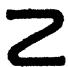
\includegraphics[keepaspectratio]{images/part002_2e6b534c.jpg}}

注。若连续同态 \(u\) 是双射，一般不能推出 \(\overline{u}\) 是单射或满射（参看习题 12）；但参看第 5 目命题 9。

\subsection{拓扑群的完备化}

一致空间 \(G_{d}\) 可以视为它的完备化 \(\hat{G}_{d}\) 的一个稠密子空间。我们将研究 G 能否被视为一个完备 Hausdorff 群 \(G'\) 的一个稠密子群。若能，则一致空间 \(G_{d}'\) 必同构于 \(\hat{G}_{d}\)（第二章 § 3 第 6 目定理 2 的推论），因而我们必须能在 \(\hat{G}_{d}\) 上定义一个拓扑群结构，它在 G 上诱导给定的拓扑群结构。因此我们必须考察：1) 能否把函数 xy 与 \(x^{-1}\) 分别连续延拓到 \(\hat{G}_{d} \times \hat{G}_{d}\) 与 \(\hat{G}_{d}\) 上；2) 这样延拓后的函数是否确实在 \(\hat{G}_{d}\) 上定义一个群结构（这时它们必然在 \(\hat{G}_{d}\) 上定义一个在 G 上诱导给定结构的拓扑群结构）。接着我们要确立：3) 当前面的运算可行时，它们所定义的拓扑群是完备的。最后，我们将看到：4) 若存在一个满足给定条件的完备群，则它在同构意义下是唯一的。

\begin{enumerate}
\def\labelenumi{\arabic{enumi})}
\tightlist
\item
  把 \(xy\) 与 \(x^{-1}\) 连续延拓。由于函数 \(xy\) 与 \(x^{-1}\) 一般不是一致连续的，我们不能应用一致连续函数的延拓定理（第二章 § 3 第 6 目定理 2）。尽管如此，凭第二章 § 3 第 6 目命题 11 以及下面的命题，我们可以延拓 \(xy\)：
\end{enumerate}

命题 6 设 \(\mathfrak{F}\) 与 \(\mathfrak{G}\) 是 \(\mathbf{G}_d\) 上的两个 Cauchy 滤子。则滤子 \(\mathfrak{F} \times \mathfrak{G}\) 在映射 \((x, y) \to xy\) 下的像是 \(\mathbf{G}_d\) 上的一个 Cauchy 滤子基。让我们估计 \(xy\) 与 \(x'y'\) 在 \(\mathbf{G}_d\) 中的“接近程度”；换言之，让我们作乘积 \((x'y')(xy)^{-1} = x'y'y^{-1}x^{-1}\)。对每个 \(a \in \mathbf{G}\)，我们还可以写 \((x'y')(xy)^{-1} = (x'a^{-1})(ay'y^{-1}a^{-1})(ax^{-1})\)。我们将看到，通过适当选取 \(a\)，只要偶 \((x, y)\) 与 \((x', y')\) 属于 \(\mathfrak{F} \times \mathfrak{G}\) 的一个充分小的集，这个乘积的三个因子中的每一个都很小。设 V 是 \(e\) 在 G 中的任一邻域；则存在一个 \(\mathbf{V}_d\)-小集 A ∈ \(\mathfrak{F}\)。在 A 中选取 \(a\)，则若 \(x\) 与 \(x'\) 是 A 的任意两点，我们有 \(x'a^{-1} \in V\) 与 \(ax^{-1} \in V\)。另一方面，关系 \(ay'y^{-1}a^{-1} \in V\) 等价于

\[
y ^ {\prime} y ^ {- 1} \in a ^ {- 1} \mathrm{V}a = \mathrm{W},
\]

而由于 W 是 e 的一个邻域，存在一个 \(W_{d}\)-小集 \(B \in \mathfrak{G}\)。于是对 A × B 中所有 \((x, y)\) 与 \((x', y')\)，我们有 \((x'y')(xy)^{-1} \in V^{3}\)，证毕。

为使 \(x^{-1}\) 可以连续延拓到 \(\hat{G}_d\) 上，充要条件是：在对称映射 \(x \to x^{-1}\) 下，一个 Cauchy 滤子（\(G_d\) 上的）的像是 \(G_d\) 上的一个 Cauchy 滤子（第二章 § 3 第 6 目命题 11）。存在一些拓扑群，这个条件在其中不满足（参看第十章 § 3 习题 16）；在本证明的余下部分我们将假设它满足。

\begin{enumerate}
\def\labelenumi{\arabic{enumi})}
\setcounter{enumi}{1}
\item
  延拓后的函数 \(xy\) 与 \(x^{-1}\) 在 \(\hat{G}_d\) 上定义一个群结构。因为若把恒等延拓原理（第一章 § 8 第 1 目命题 2 推论 1）应用于函数 \(x(yz)\) 与 \((xy)z\)（它们定义在 \(\hat{G}_d \times \hat{G}_d \times \hat{G}_d\) 上且在稠密子空间 \(G_d \times G_d \times G_d\) 上相等），我们就看出合成法则 \((x, y) \to xy\) 在 \(\hat{G}_d\) 上是结合的。出于同样的理由，函数 \(x, ex, xe\) 在 \(\hat{G}_d\) 上相同，且函数 \(e, xx^{-1}, x^{-1}x\) 在 \(\hat{G}_d\) 上相同。
\item
  拓扑群 \(\hat{\mathbf{G}}_d\) 是完备的。设 \(\mathfrak{U}_d\) 是它的右一致结构，\(\mathfrak{U}\) 是 \(\hat{\mathbf{G}}_d\) 上的由 \(\mathbf{G}\) 的右一致结构的完备化所得的一致结构。则 \(\mathfrak{U}\) 与 \(\mathfrak{U}_d\) 在 \(\mathbf{G}\) 上诱导相同的一致结构，因而每个 Cauchy 滤子基 \(\mathfrak{B}\)（\(\mathbf{G}\) 上的，关于 \(\mathfrak{U}_d\) 的）也是关于 \(\mathfrak{U}\) 的一个 Cauchy 滤子基。现在 \(\mathfrak{B}\) 在 \(\hat{\mathbf{G}}_d\) 中收敛，因为 \(\mathcal{U}\) 是一个完备一致结构；且由于 \(\mathcal{U}\) 与 \(\mathcal{U}_d\) 在 \(\hat{\mathbf{G}}_d\) 上诱导相同的拓扑，可知（第二章 § 3 第 4 目命题 9）\(\mathcal{U}_d\) 是一个完备一致结构。这个结论还表明 \(\mathcal{U}\) 与 \(\mathcal{U}_d\) 相同（第二章 § 3 第 6 目定理 2 的推论）。
\item
  唯一性。这由第 3 目命题 5 得出。
\end{enumerate}

概括起来，我们证明了下面的定理：

定理 1 Hausdorff 拓扑群 G 同构于一个完备群 \(\hat{G}\) 的一个稠密子群，当且仅当关于 G 的右一致结构的一个 Cauchy 滤子在对称映射 \(x \to x^{-1}\) 下的像是关于这个一致结构的一个 Cauchy 滤子。完备群 \(\hat{G}\)（它称为 G 的完备化）这时是唯一的（在同构意义下）。

命题 7 设 G 是一个具有完备化 \(\hat{G}\) 的 Hausdorff 拓扑群。则 G 中单位元的诸邻域在 \(\hat{G}\) 中的闭包构成 \(\hat{G}\) 中单位元的一个基本邻域系。

由于 \(\hat{G}\) 是正则的，\(\hat{G}\) 中单位元的每个邻域含有 e 在 \(\hat{G}\) 中的一个开邻域 U 的闭包 V，而 V 也是 U 在 G 上的迹的闭包。

设 G 是一个未必 Hausdorff 的群；设 \(N = \overline{e}\)，\(G' = G/N\) 是伴随于 G 的 Hausdorff 群（§ 2 第 6 目）。若 \(G'\) 有一个完备化 \(\hat{G}'\)，这个完备化称为 G 的 Hausdorff 完备化，记作 \(\hat{G}\)；这时 \(\hat{G}_{d}'\)（相应地 \(\hat{G}_{s}'\)）是一致空间 \(G_{d}\)（相应地 \(G_{s}\)）的 Hausdorff 完备化（第二章 § 3 第 7 目）。

命题 8 设 G 是一个具有 Hausdorff 完备化 \(\hat{G}'\) 的拓扑群。则 G 到一个完备 Hausdorff 群 H 中的每个连续同态 \(u\) 可以唯一地分解为 \(u = v \circ \varphi\)，其中 \(v\) 是 \(\hat{G}'\) 到 H 中的一个连续同态，而 \(\varphi\) 是 G 到 \(\hat{G}'\) 中的典范映射（G' 到 \(\hat{G}'\) 中的典范单射与 G 到 G/N = G' 上的典范同态 \(\psi\) 的复合）。

由于 \(u\) 的核是闭的且含有 \(e\)，它含有 \(N\)，因而 \(u\) 可以写作 \(u = w \circ \psi\)，其中 \(w\) 是 \(G'\) 到 \(H\) 中的一个连续同态；现在对 \(w\) 应用第 3 目命题 5。

\subsection{交换拓扑群的一致结构与完备化}

我们已经指出，在交换拓扑群 G 上左一致结构与右一致结构相同；每当我们谈到 G 的一致结构时，所指的就是这个唯一的一致结构。

定理 2 设 G 是一个交换拓扑群。则函数 \(x^{-1}\) 与 xy 分别在 G 与 G × G 上一致连续。此外 G 容许一个 Hausdorff 完备化 \(\hat{G}\)，且 \(\hat{G}\) 是交换的。

\(x^{-1}\) 的一致连续性由第 1 目命题 2 得出，而 xy 的一致连续性由第 1 目命题 3 得出，因为 \((x, y) \to xy\) 是 \(G \times G\) 到 G 中的一个连续同态。若 G 是 Hausdorff 的，它满足第 4 目定理 1 的条件（如同每个左一致结构与右一致结构相同的 Hausdorff 群一样）；此外由恒等延拓原理，函数 xy 与 yx 在 \(\hat{G} \times \hat{G}\) 上相等；由此得到定理的第二部分，办法是在一般情形考虑伴随于 G 的 Hausdorff 群。

特别地，由这个定理可得：若 \(f\) 与 \(g\) 是一致空间 \(\mathbf{X}\) 到一个交换群 \(G\)（以加法记的）中的两个一致连续映射，则函数 \(-f\) 与 \(f + g\) 是一致连续的。

命题 9 设 G 是一个交换群，\(\mathfrak{T}_1\)、\(\mathfrak{T}_2\) 是与 G 的群结构相容的两个 Hausdorff 拓扑。设 \(\mathfrak{T}_1\) 比 \(\mathfrak{T}_2\) 细，且存在关于 \(\mathfrak{T}_1\) 的 o 的一个基本邻域系，它的成员对 \(\mathfrak{T}_2\) 是闭的。设 \(\mathrm{G}_1, \mathrm{G}_2\) 分别是 G 关于拓扑 \(\mathfrak{T}_1, \mathfrak{T}_2\) 的完备化，\(f: \mathrm{G}_1 \to \mathrm{G}_2\) 是延拓 G 的恒等映射的连续同态（第 3 目命题 5）。则 \(f\) 是单射。

设 G 以加法记。设 \(\mathfrak{U}_{1}\) 是 G 上（依第 1 目）对应于拓扑 \(\mathfrak{T}_{1}\) 的一致结构：只需证明若 F 与 \(F'\) 是关于 \(\mathfrak{U}_{1}\) 的两个极小 Cauchy 滤子（第二章 § 3 第 2 目），它们在 \(G_{2}\) 中收敛于同一点 a，则 \(F = F'\)（第二章 § 3 第 7 目）。为此，只需证明 \(F \cap F'\) 是关于 \(\mathfrak{U}_{1}\) 的一个 Cauchy 滤子。设 V 是 G 中关于 \(\mathfrak{T}_{1}\) 的 o 的一个邻域，使得 V 在 \(\mathfrak{T}_{2}\) 中是闭的，又设 W 是 G 中关于 \(\mathfrak{T}_{1}\) 的 o 的一个对称邻域，使得 \(W + W \subset V\)。由假设，存在一个 \(W_{d}\)-小集 M（相应地 \(M'\)），它属于 F（相应地 \(F'\)）；若 \(x \in M\) 且 \(y \in M\)，我们有 \(y - x \in W\)，即 \(y \in x + W\)。若 \(\overline{W}\) 与 \(\overline{V}\) 是 W 与 V 在 \(G_{2}\) 中的闭包，则由此可得 \(y \in x + \overline{W}\)，因而由于 a 在 M 的闭包中，\(a \in x + \overline{W}\) 对每个 \(x \in M\) 成立。类似地，\(a \in x' + \overline{W}\) 对每个 \(x' \in M'\) 成立，于是 \(x - x' \in \overline{W} + \overline{W}\)；但由 \((x, y) \to x + y\) 是 \(G_{2} \times G_{2}\) 到 \(G_{2}\) 中的一个连续映射，我们有 \(\overline{W} + \overline{W} \subset \overline{W + W} \subset \overline{V}\)。由此可得，若 \(x \in M\) 且 \(x' \in M'\)，则 \(x - x' \in \overline{V} \cap G = V\)，因为 V 在 \(\mathfrak{T}_{2}\) 中是闭的；证毕。

推论 1 在命题 9 的假设下，若 A 是 G 的一个子集，它关于一致结构 \(\mathfrak{U}_{2}\)（对应于 \(\mathfrak{T}_{2}\) 的）是一个完备子空间，则 A 关于一致结构 \(\mathfrak{U}_{1}\)（对应于 \(\mathfrak{T}_{1}\) 的）也是一个完备子空间。

若 \(A_{1}\) 是 A 在 \(G_{1}\) 中的闭包，则 \(f(A_{1})\) 含于 A 在 \(G_{2}\) 中的闭包，而由假设这个闭包等于 A。由于依定义 \(f(A)=A\) 且 f 是单射，我们有 \(A_{1}=A\)。

推论 2 设 G 是一个交换群，\(\mathfrak{T}_1, \mathfrak{T}_2\) 是与 G 的群结构相容的两个拓扑。设 \(\mathfrak{T}_1\) 比 \(\mathfrak{T}_2\) 细，且存在 o 的一个基本邻域系 \(\mathfrak{B}\)（关于 \(\mathfrak{T}_1\) 的），它的成员关于一致结构 \(\mathfrak{U}_2\)（对应于 \(\mathfrak{T}_2\) 的）是完备的。则 G 关于一致结构 \(\mathfrak{U}_1\)（对应于 \(\mathfrak{T}_1\) 的）是完备的。

\(\mathfrak{B}\) 中的诸集在拓扑 \(\mathfrak{T}_{2}\) 中是闭的，因而由推论 1 关于一致结构 \(\mathfrak{U}_{1}\) 是完备的；于是结论由第 3 目命题 4 得出。

\section{逆紧作用于拓扑空间的群；拓扑群与带算子空间中的紧性}

\subsection{逆紧作用于拓扑空间的群}

定义 1 设 G 是连续作用在拓扑空间 X 上的一个拓扑群。如果映射

\[
\theta : (s, x) \rightarrow (x, s. x) \text{ 从 } \mathbf{G} \times \mathbf{X} \text{ 到 } \mathbf{X} \times \mathbf{X}
\]

是逆紧的（第一章 § 10 第 1 目定义 1），就称 G 逆紧作用在 X 上。

设 \(\Gamma \subset \mathbf{G} \times \mathbf{X} \times \mathbf{X}\) 是映射 \(\rho: (s, x) \to s.x\) 的图。由于 \(\rho\) 连续，映射 \(\sigma: (s, x) \to (s, x, s.x)\) 是 \(\mathbf{G} \times \mathbf{X}\) 到 \(\Gamma\) 上的一个同胚，且复合映射

\[
\mathbf {G} \times \mathbf {X} \xrightarrow {\sigma} \Gamma \xrightarrow {\mathrm{pr} _ {2 3}} \mathbf {X} \times \mathbf {X}
\]

就是 \(\theta\)。因此定义 1 等价于说 \(\operatorname{pr}_{23}\) 在 \(\Gamma\) 上的限制是 \(\Gamma\) 到 \(\mathbf{X} \times \mathbf{X}\) 中的一个逆紧映射。

第一章 § 10 第 2 目定理 1 表明，G 逆紧作用在 X 上，当且仅当下列条件满足：

对每个由超滤子 F 过滤的集 A，以及每个映射

\[
\alpha \rightarrow (s _ {\alpha}, x _ {\alpha})
\]

（A 到 \(\mathbf{G} \times \mathbf{X}\) 中的），如果映射 \(\alpha \to (s_{\alpha}.x_{\alpha}, x_{\alpha})\) 有一个极限 \((b, a)\)（关于 \(\mathfrak{F}\) 的），则 \(\alpha \to s_{\alpha}\) 有一个极限 \(t \in \mathbf{G}\)（关于 \(\mathfrak{F}\) 的），使得 \(t.a = b\)。

例。1) 设 H 是拓扑群 G 的一个闭子群。若 G 逆紧作用在 X 上，则 H 也逆紧作用在 X 上，因为 H × X 在 G × X 中是闭的（第一章 § 10 第 1 目命题 5 推论 1）。例如若取 X = G，G 通过左平移作用在自身上，则映射 G × X → X × X 是一个同胚，因而是逆紧的；于是 H 通过左平移逆紧作用在 G 上。

\begin{enumerate}
\def\labelenumi{\arabic{enumi})}
\setcounter{enumi}{1}
\tightlist
\item
  若 G 逆紧作用在 X 上，则它逆紧作用在 X 的每个子空间 \(X'\)（它是 X 的点的轨道的并）上（换言之，\(X'\) 关于由 G 定义的等价关系是饱和的）。因为 \(X' \times X'\) 在 \(G \times X\) 中的原像是 \(G \times X'\)，且我们可以应用第一章 § 10 第 1 目命题 3。
\end{enumerate}

命题 1 设 G 是连续作用在拓扑空间 X 上的一个拓扑群，K 是 G 的一个拟紧子集。则映射 \(\rho: (s, x) \to s.x\)（\(K \times X\) 到 \(X\) 中的）是逆紧的。

\(\rho\) 分解为 \(\mathbf{K} \times \mathbf{X} \to \mathbf{K} \times \mathbf{X} \xrightarrow{\mathrm{pr}_2} \mathbf{X}\)，其中 \(\alpha(s, x) = (s, s.x)\)。\(\alpha\) 是一个同胚，因为 \(\alpha^{-1}: (s, y) \to (s, s^{-1}.y)\) 连续。由于 \(\mathbf{K}\) 是拟紧的，\(\mathrm{pr}_2\) 是逆紧的（第一章 § 10 第 2 目定理 1 推论 5）；因而 \(\rho\) 是逆紧的（第一章 § 10 第 1 目命题 5）。

推论 1 若 A 是 X 的一个闭（相应地紧）子集，则 K.A 在 X 中是闭的（相应地，若 X 是 Hausdorff 的，则是紧的）。

关于闭集的断言由命题 1 以及逆紧映射是闭映射这一事实（第一章 § 10 第 1 目命题 1）得出。关于紧集的断言是显然的。

\pandocbounded{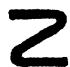
\includegraphics[keepaspectratio]{images/part002_62417fce.jpg}}

应当注意，若 L 是 X 的一个紧子集，F 是 G 的一个闭子集，则 F. L 在 X 中未必是闭的（§ 2 习题 29；参看第 5 目命题 12 的推论）。

推论 2 若 K 是拓扑群 G 的一个拟紧子群，则等价关系 \(x^{-1}y \in K\) 是闭的，且典范映射 \(\varphi: G \to G/K\) 是逆紧的。

第一个断言由推论 1 应用于通过右平移作用在自身上的 G 得出，第二个断言则由第一章 § 10 第 2 目定理 1 得出。

推论 3 设 K 是拓扑群 G 的一个拟紧正规子群，\(\varphi\) 是典范映射 G → G/K。则对 G 的每个闭子群 A，A/A∩K 到 \(\varphi(A)\) 上的典范双射是拓扑群的一个同构。

由于 \(x^{-1}y \in K\) 是一个闭等价关系（推论 2），本推论由第一章 § 5 第 2 目命题 4 得出。

命题 2 设 K 是连续作用在 Hausdorff 空间 X 上的一个紧群。则：

\begin{enumerate}
\def\labelenumi{\alph{enumi})}
\item
  K 逆紧作用在 X 上。
\item
  映射 \((s, x) \to s.x\)（\(\mathbf{K} \times \mathbf{X}\) 到 \(\mathbf{X}\) 中的）是逆紧的。
\item
  X 到 X/K 上的典范映射是逆紧的。
\item
  是命题 1 的推论。至于 a)，由于 K 是紧的，\(\operatorname{pr}_{2}:(s,x)\to x\) 是逆紧的（第一章 § 10 第 2 目定理 1 推论 5）；因而，由于 X 是 Hausdorff 的，\((s,x)\to(x,s.x)\) 是逆紧的（第一章 § 10 第 1 目命题 5 推论 3）。剩下证明 c)。依命题 1 的推论 1，典范映射 \(\varphi:X\to X/K\) 是闭的。若 Z 是任一拓扑空间且让 K 平凡作用在 Z 上，则 K 连续作用在 \(X\times Z\) 上，因而典范映射 \(X\times Z\to(X\times Z)/K\) 是闭的。但 \((X\times Z)/K\) 可以典范地等同于 \((X/K)\times Z\)（§ 2 第 4 目引理 2 及第一章 § 5 第 3 目命题 8 的推论）；因而典范映射 \(X\times Z\to(X\times Z)/K\) 可以等同于 \(\varphi\times1\)，且由于它对所有 Z 是闭的，可知 \(\varphi\) 是逆紧的。
\end{enumerate}

推论 1 在命题 2 的假设下，X 是紧的（相应地局部紧的），当且仅当 X/K 是紧的（相应地局部紧的）。

这由典范映射 \(X \rightarrow X/K\) 是逆紧的这一事实得出，依据第一章 § 10 第 4 目命题 9。

推论 2 设 G 是一个 Hausdorff 拓扑群，K 是 G 的一个紧子群。则 G 是紧的（相应地局部紧的），当且仅当 G/K 是紧的（相应地局部紧的）。

对通过右平移作用在 G 上的 K 应用推论 1。
